\RequirePackage{ifluatex}
\let\ifluatex\relax

\documentclass[aps,%
12pt,%
final,%
oneside,
onecolumn,%
musixtex, %
superscriptaddress,%
centertags]{article} %% 
\topmargin=-40pt
\textheight=650pt
\usepackage[english,russian]{babel}
\usepackage[utf8]{inputenc}
%всякие настройки по желанию%
\usepackage[colorlinks=true,linkcolor=black,unicode=true]{hyperref}
\usepackage{euscript}
\usepackage{supertabular}
\usepackage[pdftex]{graphicx}
\usepackage{amsthm,amssymb, amsmath}
\usepackage{textcomp}
\usepackage[noend]{algorithmic}
\usepackage[ruled]{algorithm}
\usepackage{lipsum}
\usepackage{indentfirst}
\usepackage{babel}
\usepackage{pgfplots}
\usepackage{setspace}
\linespread{1.2}
\pgfplotsset{compat=1.9}
\selectlanguage{russian}
\pgfplotsset{model/.style = {blue, samples = 100}}
\pgfplotsset{experiment/.style = {red}}
\theoremstyle{plain}
\binoppenalty=10000
\newtheorem{theorem}{Теорема}[section] %
\setlength{\parindent}{2.4em}
\setlength{\parskip}{0.1em}
%\renewcommand{\baselinestretch}{1.0}
\theoremstyle{definition}
\newtheorem{definition}{Определение}[subsection]
\theoremstyle{remark}
\newtheorem{remark}{Замечание}[section]

\newtheorem{corollary}{Следствие}
\newtheorem{proposition}{Proposition}
\newtheorem{example}{Пример}
\renewcommand*{\proofname}{Proof}

\newtheorem{lemma}{Лемма}[section]

\graphicspath{ {./image/} }
\usepackage{xcolor}
\usepackage{hyperref}


\begin{document}

\begin{titlepage} 
\begin{center}
% Upper part of the page
%\textbf{\Large САНКТ-ПЕТЕРБУРГСКИЙ ГОСУДАРСТВЕННЫЙ ЭКОНОМИЧЕСКИЙ УНИВЕРСИТЕТ} \\[1.0cm]
%\textbf{\large Кафедра Прикладной Математики и Информатики}\\[3.5cm]
 
% Title
\textbf{}\\[10.0cm]
\textbf{\LARGE Методы прогнозирования. Билеты}\\[0.5cm]
\textbf{\Large Александр Широков ПМ-1701} \\[0.2cm]

%supervisor
\begin{center} \large
{Преподаватель:} \\[0.5cm]
\textsc {Ивахненко Дарья Александровна}\\
\end{center}
% \begin{flushright} \large
%\emph{Рецензент:} \\
%д.ф. - м.н., профессор \textsc{Надеемся Нам Помогут}
%\end{flushright}
%\begin{flushright} \large
%\emph{Заведующий кафедрой:} \\
%д.ф. - м.н., профессор \textsc{Не Обмани Себя}
%\end{flushright}
\vfill 

% Bottom of the page

{\large {Санкт-Петербург}} \par
{\large {2020 г., 6 семестр}}
\end{center} 
\end{titlepage}

% Table of contents
\begin{thebibliography}{3}
	\bibitem{A}
	GLM An Applied Approach, Ulf Olsson
\end{thebibliography}
\tableofcontents
\newpage

\section{Понятие прогноза и прогнозирования. Компоненты уровня динамического ряда}

\subsection{Понятие временного ряда, прогноза и прогнозирования}

\begin{definition}
	\textbf{Временной ряд}  - последовательность значений признака $y$, измеряемого через постоянные временные интервалы:
	$$y_1, y_2,\ldots, y_T, \qquad y_t \in R$$
\end{definition}

\begin{center}
	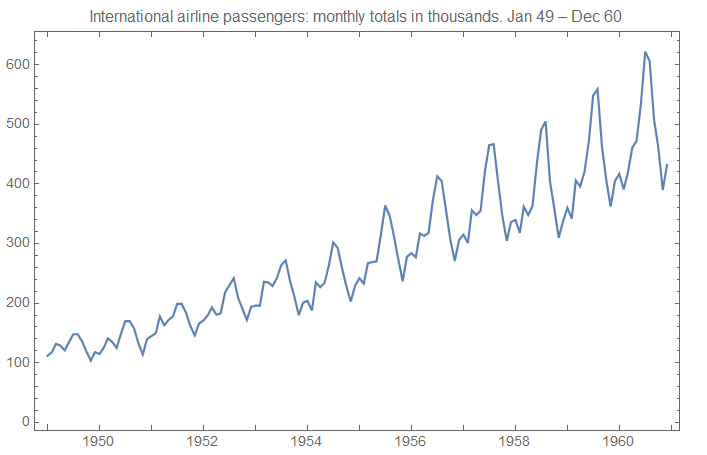
\includegraphics[scale=0.6]{images/1.png}
	Рис. 1: Временной ряд
\end{center}
\textbf{Задача прогнозирования} состоит в нахождении функции $f_T$:
$$y_{T+h} \approx f_T(y_T,\ldots,y_1,h) \equiv \hat{y}_{T+h|T}$$
где $h \in \{1,2,\ldots,H\}$, $H$ - горизонт прогнозирования

\begin{definition}
	\textbf{Предсказательный интервал} - интервал, в котором предсказываемая величина окажется с вероятностью не меньше заданной.
\end{definition}

\newpage
\subsection{Компоненты уровня динамического ряда}

Поведение временных рядов можно описать следующими характеристиками:

\begin{itemize}
	\item \textbf{Тренд} - плавное долгосрочное изменение уровня ряда. 

	Тренд отражает общее направление временного ряда, он может быть повышающимся, понижающимся или постоянным. Тренд может увеличиваться или уменьшаться различными способами (линейно, экспоненциально).

	\item \textbf{Сезонность} - циклические изменения уровня ряда с постоянным периодом.

	Сезонность фиксирует эффекты, которые происходят с определенной частотой. Это можт быть обусловлено большим количеством факторов, например, сезонность, связанная со сменой времен года и.т.д

	\item \textbf{Ошибка} (остатки, случайная компоненты) - непрогнозируемая случайная компонента ряда.

	Остатки - это оставшиеся случайные колебания, после того, как тренд и сезонность удаляются из оригинального временного ряда. В остатках мы \textit{не должны видеть тендценцию или сезонность}, так как остатки представляют собой краткосрочные колеабния. Остатки либо случайные, либо являются частью компонентов тренда и сезонности, которые \textit{были пропущены при разложении} временного ряда.

	Соответственно, вид остатков показывает, содержится ли в остатках большая часть информации, которая не была учтена и можно ли построить более сложную модель, которая будет лучше описывать имеющиеся данные.

	\item \textbf{Цикл} - изменения уровня ряда с переменным периодом (экономические циклы, периоды солнечной активности)

	\item \textbf{Разладка} - смена модели ряда.
\end{itemize}

\begin{definition}
	\textbf{Аддитивная модель} - наблюдаемый временной ряд является суммой его компонент - тренда $T$, сезонности $S$ и ошибки $E$:
	$$TS = T + S + E$$

	Модель является аддитивной, если сезонные колебания и остаточная ошибка колеблятся вместе с изменением тренла и если амплитуда колебаний значений ряда вокргу тренда примерно одинаковая
\end{definition}

\begin{definition}
	\textbf{Мультипликативная модель} - мультипликативные модели предполагают, что наблюдаемый временной ряд является \textbf{произведением его компонент}:
	$$TS = T \cdot S \cdot E$$

	В случае, когда сезонные колебания изменяются пропорционально уровню ряда, говорят о мультипликативной сезонности.
\end{definition}

\newpage

\section{Автокорреляция. Коррелограмма. Частичная автокорреляция}

\subsection{Автокорреляция}

Ряд может содержать, помимо случайной составляющей, либо тенденцию, либо только сезонную компоненту, либо все компоненты вместе. Для того, чтобы выявить наличие той или иной неслучайной компоненты, исследуется корреляционная зависимость между последовательными уровнями временного ряда или \textbf{автокорреляция уровней ряда}.

Основная идея - при наличии тенденции и циклических колебаний, значения каждого последующего уровня ряда зависят от предыдущих.

\begin{definition}
	\textbf{Автокорреляция} - количественная характеристика сходства между значениями ряда в соседних точках.  Автокорреляционная функция задается следующим соотношением:
	$$r_{\tau} = \frac{E(y_t-Ey)(y_{t+\tau}-Ey)}{Dy}$$
\end{definition}

Коэффициент автокорреляции уровней ряда \textit{первого порядка} измеряет зависимость между соседними уровнями ряда $t$ и $t-1$, то есть при \textit{лаге} $1$.

Если значение коэффициента автокорреляции близко к единице, это указывает на очень тесную зависимость между соседними уровнями временного ряда и о наличии во временном ряде сильной линейной тенденции, так как автокорреляция - это \textit{корреляци Пирсона - выборочного коэффициента корреляции} между исходным рядом и его версией, сдвинутой на несколько отсчетов.

Аналогично определяются коэффициенты автокорреляции более высоких порядков:
$$r_{\tau} = \frac{\sum\limits_{t=1}^{T-\tau} (y_t - \bar{y})(y_{\tau+t} - \bar{y})}{\sum\limits_{t=1}^T (y_t - \bar{y})^2}$$
$$r_{\tau+1} = \frac{\sum\limits_{t=\tau}^{T} (y_t - \bar{y})(y_{t-\tau} - \bar{y})}{\sum\limits_{t=1}^T (y_t - \bar{y})^2}$$
где $T$ - длина временного ряда.

\begin{definition}
	Количество отсчетов, на которое сдвинут ряд, называется \textit{лагом автокорреляции $\tau$} (число периодов, по которым рассчитывается коэффициент автокорреляции)
\end{definition}

Автокорреляция часто приводит к какому-то известному нам виду графика, тогда как временной ряд без автокорреляции будет проявлять случайность.

\textbf{Свойства автокорреляции}

1. Коэффициент автокорреляции строится по аналогии с линейным коэффициентом корреляции, поэтому он характеризует тесноту \textit{только линейной связи} текущего и предыдущего уровня. Для временных рядов с нелинейной тенденции, коэффициент автокорреляции будет близок к $0$, хотя тенденция все же в ряде есть.

2. По знаку коэффициента автокорреляции \textit{нельзя} делать выпод о возрастающей или убывающей тенденции в уровнях ряда.

\begin{definition}
	Последовательность коэффициентов автокорреляции уровней различных порядков, начиная с первого, называется \textit{автокорреляционной функцией временного ряда} (\textbf{ACF}).
\end{definition}

\newpage
\subsection{Коррелограмма}

\begin{definition}
	График зависимости автокорреляционной функции от величины лага называется \textit{коррелограммой}.
\end{definition}

\begin{center}
	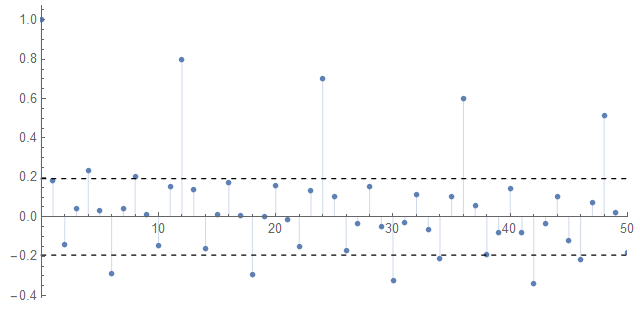
\includegraphics[scale=0.6]{images/2.png}
	Рис. 2: Коррелограмма
\end{center}

С помощью коррелограммы удобно анализировать при разных значениях лага величину автокорреляции. По оси ординат откладывается автокоореляции, по оси абцисс - размер лага $\tau$.

Анализ автокорреляционной функции позволяет определить лаг, при котором автокорреляция наиболее высокая, лаг, при котором связь между текущим и предыдущим уровнями ряда наиболее тесная.

\subsubsection{Значимость автокорреляции}

На коррелогрмме помимо значений автокорреляции также изображен коридор вокруг горизонтальной оси.

Это коридор \textit{значимости отличия корреляции от нуля}. Как и для обычной корреляции Пирсона, значимость вычисляется при помощи критерия Стьюдента.

В качестве нулевой гипотезы предполагают, что $H_0: r_{\tau} = 0$. Альтернативной гипотезой является двустороння гипотеза о том, что $H_1: r_{\tau} < \neq > 0$, потому что при анализе временных рядов крайне редко имеется гипотеза о том, какой по знаку должна быть корреляция - положительной или отрицательной. 

Статистическую значимость $r_{\tau}$ можно определить с помощью $t$-критерия:
$$T(y) = \frac{r_{\tau}}{\sqrt{1-r_{\tau}^2}} \cdot \sqrt{T-\tau-2} \sim t(T-\tau-2)$$

Если $T(y) > t_{table}(T-\tau-2)$, то принято сичтать, что корреляция статистически значима.

То есть значения автокорреляции, выходящие за пределы коридора вокруг горизонтальной оси, явлются статистически значимыми, а значения внутри коридора - \textit{статистически  незначимы}

\subsubsection{Анализ коррелограммы}

1. Если наиболее высоким является коэффициент автокорреляции первого порядка, то исследуемый ряд содержит \textit{только тенденцию}.

2. Есди наиболее высоким оказался коэффициент автокорреляции \textit{второго порядка}, то ряд содержит циклические колебания с циклом, равным двум периодам времени, то есть имеет \textit{пилообразную структуру}.

3. Если наиболее высоким оказался коэффициент автокорреляции порядка $\tau$, то ряд содержит циклические колебания с периодичностью в $\tau$ моментов времени.

4. Если ни один из коэффициентов $\tau$ не является значимым, то либо ряд не содержит тенденции и циклических колебаний и имеет только случайную составляющую, либо содержит сильную нелинейную связь, для исследования которой нужно провести дополнительный анализ.

\subsubsection{Диаграмма рассеяния}

Если построить график зависимости $y_t$ от $y_{t+1}$, то такой график будет называться \textbf{диаграммой рассеивания}. Если рассмотреть продажи в одни и те же месяцы соседних лет, то точки на графике стягиваются к главной диагонали. Это значит, что значения в одни и те же месяцы соседних лет сильно похожи:

\begin{center}
	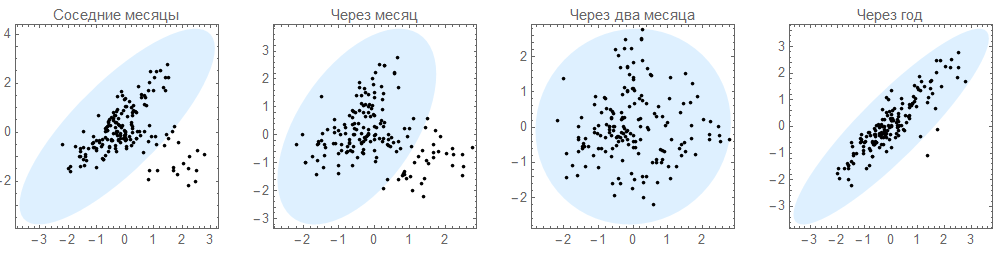
\includegraphics[scale=0.33]{images/5.png}

	Рис. 5: Различные диаграммы рассеивания, на последнем рисунке видна линейная тесная связь
\end{center}

% Чем ближе точки стягиваются к главной диагонали, тем сильнее линейная связь.

\newpage
\section{Понятие стационарности}

\begin{definition}
	\textbf{Стационарный временной ряд} - такой временной ряд $y_1,\ldots, y_T$, в которой свойства ряда не зависят от времени, то есть $\forall k$ (ширина окна) распределение $y_t,\ldots,y_{t+k}$ не зависит от времени.
\end{definition}

Данный ряд обладает следующими особенностями, следующими из определения:

\begin{itemize}
	\item \textbf{Постоянное среднее значение}, то есть у стационарного ряда \textit{нет тренда}
	\item \textbf{Постоянная дисперсия} (гомоскедастичность), то есть дисперсия не зависит от другой случайной величины. Если дисперсия не постоянна и зависит от предыдущих наблюдений, то ряд нестационарен 
	\item \textbf{Постоянная автокорреляционная структура}, то есть значения автокорреляции незначимы - отсутствует линейная связь с предыдущими значениями.
	\item \textbf{Отсутствие сезонности}, ведь если ширина окна меньше сезонного периода, то распределение будет разным, в зависимости от положения окна.
\end{itemize}

\textbf{Замечание}: ряды в которых есть непериодические циклы, не обязательно являются нестационарными.

Почему же стационарность настолько важна? Стационарность является фундаментальным предположением в большинстве случаев прогнозирования моделей временных рядов:

\begin{itemize}
	\item Без стационарности множество базисных моделей временных рядов попросту не работали бы
	\item Преобразования могут применяться для преобразования нестационарного временного ряда в стационарный перед моделированием, например, поведения ряда или прогноза.
\end{itemize}

По стационарному ряду просто строить прогноз, так как предполагается, что его будущие характеристики не будут отличаться от наблюдаемых текущих.

\newpage
\subsection{Способы определения стационарности ряда}

Для того, чтобы определить, является ли ряд стационарным, можно использовать несколько способов:

\begin{itemize}
	\item Построение графика

	С самого начала необходимо построить \textbf{график} временного ряда. Обычно, данного шага достаточно для определения, является ли ряд нестационарным, потому что видно либо наличие сезонности, либо тренда, либо автокорреляции, либо непостоянство дисперсии, которую необходимо стабилизировать.
	\item Оценка с помощью статистик

	Вычисления \textbf{математических ожиданий и дисперсий} на протяжении всего временного ряда является важным способом определения, в каких моментах ряд является стационарным. Легким способом является \textbf{разделение временного ряда} на \textit{несколько временных периодов} и \textit{подсчет} статистических значений на данных промежутках.

	\textbf{Большие отклонения в среднем или дисперсии} между различными промежутками означает, что данные \textit{нестационарны}. 

	Если мы хотим еще более уточнить, то можем воспользоваться тестами, чтобы определить, является ли разница в среднем или разница в отклонениях статистически значимой.
	\item Гистограмма

	\textbf{Гистограмма} дает хорошие предположения о виде ряда. Если распределение похоже на \textit{нормальное}, то ряд практически наверняка является \textit{стационарным}.
	\item Тест Дики-Фуллера

	Гипотезу о стационаности можно проверить с помощью критерия Дики-Фуллера. Статистику данного критерия рассмотрим чуть позже.
\end{itemize}

\newpage
\subsection{Преобразование ряда в стационарный}

Существует несколько способов преобразования нестационарного ряда в стационарный:

\begin{itemize}
	\item Убрать тренд
	\item Привести ряд к ряду с постоянной дисперсией путем логарифмирования
	\item Убрать автокорреляцию путем диффенцирования ряда
	\item Убрать сезонность
\end{itemize}

Зачастую приходится делать несколько из данных преобразований в одном наборе данных. Рассмотрим последовательно каждое из преобразований.

\subsubsection{Стабилизация дисперсии. Преобразование Бокса-Кокса}

Если во временном ряде \textbf{монотонно по времени изменяется дисперсия}, то применяется специальное преобразование, стабилизирующее дисперсию. Часто в качестве такого преобразования модно использовать простое логарифмирование.

В результате логарифмирования размер колебаний в начале и конце ряда становится очень похожим и дисперсия стабилизируется.

\begin{center}
	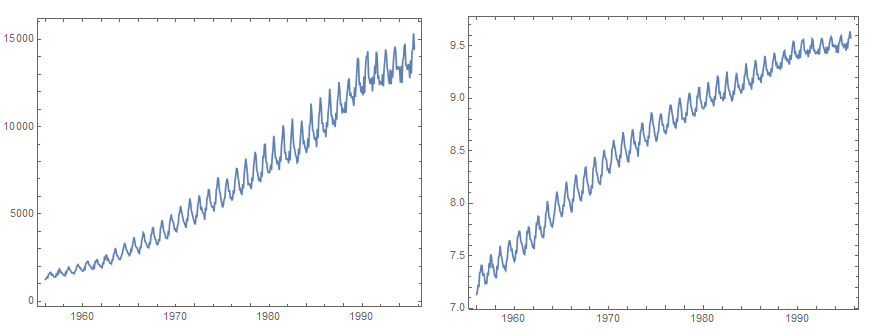
\includegraphics[scale=0.5]{images/3.png}
	Рис. 4: Слева - исходный ряд, справа - логарифмированный
\end{center}

Логарифмирование принадлежит к параметрическому семейству \textit{преобразований Бокса-Кокса.} В случае, когда значения ряда $y>0$, преобразование Бокса-Коса имеет вид:
$$y^{(\lambda)} = 
\left\{
\begin{matrix}
\frac{y^{\lambda}-1}{\lambda}, \lambda \neq 0 \\
\ln y, \lambda = 0
\end{matrix} \right. $$

Заметим, что экспонента может быть разложена в ряд Тэйлора:
$$e^x = 1 + \sum\limits_{n=1}^{\infty} \frac{x^n}{n!} = 1 + x + \frac{x^2}{2!} + \ldots $$
поэтому:
$$y^{(\lambda)} = e^{\lambda \ln y} = 1 + \lambda \ln y + O((\lambda \ln y)^2)$$
и получаем, что $y^{(\lambda)} = \ln y$ для $\lambda \to 0$.

Параметр $\lambda$ определяет, как будет преобразован ряд. Если $\lambda = 0$, то будет произведено логарифмирование, если $\lambda =1$ - тождественное преобразование со смещением на единицу, при других $\lambda$ - степенное преобразование.

Значение параметра $\lambda$ применяется так, чтобы дисперсия была как можно более стабильной во времени. Так, параметр $\lambda$ выбирается методом максимального правдоподобия. 

Найдем функцию правдоподобия:

\begin{proof}
	$$ L = \prod_{i=1}^{T} {\frac{1}{\sqrt{2\pi}\cdot \sigma}} \cdot \exp \left ( {-\frac{({y_i^{(\lambda)} - \overline{y}^{(\lambda)})^2}}{\sigma^2}}\right) \cdot J(\lambda,y) \to \max $$

	Прологорифмируем:
	$$ \ln L = \sum_{i=1}^{T} \left ( \ln \frac{1}{\sqrt{2\pi}\cdot \sigma}  - \frac{({y_i^{(\lambda)} - \overline{y}^{(\lambda)})^2} }{2\sigma^2} + \ln J(\lambda,y) \right )  $$

	Воспользуемся оценкой выборочной дисперсии:
	$$ \hat{\sigma}^2 = \sum_{i=1}^{T} \frac{({y_i^{(\lambda)} - \overline{y}^{(\lambda)}})^2}{T} $$
	$$ \ln \frac{1}{\sqrt{2\pi \sigma^2}} = \ln \frac{1}{\sqrt{2\pi}} + \ln \frac{1}{\sqrt {\sigma^2}} = \ln \frac{1}{\sqrt{2\pi}} - \ln \frac{({y_i^{(\lambda)} - \overline{y}^{(\lambda)}})^2}{T}$$ 

	Тогда:
	$$ \ln L = \sum_{i=1}^{T} \ln \frac{1}{\sqrt{2\pi}} - \ln \frac{({y_i^{(\lambda)} - \overline{y}^{(\lambda)}})^2}{T} - \frac{T}{2} + \log \prod_{i=1}^{T} y_{i}^{\lambda - 1} = $$ 
	$$ = \sum_{i=1}^{T} \ln \frac{1}{\sqrt{2\pi}} - \sum_{i=1}^{T} \ln \frac{({y_i^{(\lambda)} - \overline{y}^{(\lambda)}})^2}{T} - \frac{T}{2} + (\lambda - 1) \sum_{i=1} \ln y_{i} =$$
	$$=  -\frac{T}{2} \cdot \ln \sum_{i=1}^{T} \frac{({y_i^{(\lambda)} - \overline{y}^{(\lambda)}})^2}{T} + (\lambda - 1) \sum_{i=1} \ln y_{i} $$

	Итого: логафрим функции правдоподобия Бокса-Кокса:

	$$ \ln L = -\frac{T}{2} \cdot \ln \sum_{i=1}^{T} \frac{({y_i^{(\lambda)} - \overline{y}^{(\lambda)}})^2}{T} + (\lambda - 1) \sum_{i=1} \ln y_{i} $$

	где $$\overline{y}^{(\lambda)} = \frac{1}{T} \sum y_i^{(\lambda)} $$

	$ T $ - количество элементов в выборке.

	Взяв производную по параметру $\lambda$ и прировняв к нулю, найдем решение, получим оценку методом максимального правдоподобия.
\end{proof}

Если ряд содержит отрицательные значения, то можно переписать правила преобразования следующим образом:
$$y^{(\lambda)} = 
\begin{cases}
\frac{(y+\lambda_2)^{\lambda}-1}{\lambda}, \lambda \neq 0 \\
\ln (y+\lambda_2), \lambda = 0
\end{cases}  , \qquad y > \lambda_2$$

При возвращении к исходному ряду важно и проделывать \textit{обратное преобразование Бокса-Кокса:}
$$y^{(\lambda)} = 
\begin{cases}
e^y \cdot  \frac{\ln (\lambda \cdot y) + 1}{\lambda}, \lambda \neq 0 \\
e^y, \lambda = 0
\end{cases}  $$

\subsubsection{Дифференцирование}

Как было сказано ранее, дифференцирование - один из способов привести ряд к стационарному, убрав из него автокорреляцию. 

\begin{definition}
	\textbf{Дифференцирование} - переход к попарным разностям соседних значений:
	$$y_t' = y_t - y_{t-1}$$

	Мы вычитаем прошлую стоимость, отсоящую от нынешней на, допустим, $1$ день, как в формуле выше.
\end{definition}

Данная операция позволяет стабилизировать среднее значение ряда и избавиться от тренда, а иногда даже от сезонности. Дифференцирование можно применять неоднократно: от ряда первых разностей, продифференцировав его, можно прийти к ряду вторых разностей и.т.д.

Длина ряда, соответственно, буедт сокращаться на величину порядка разностей, но при этом мы добьемся стационарности.

\begin{definition}
	\textbf{Сезонное дифференцирование ряда} - переход к попарным разностям в соседних сезонах. Если длина периода сезонности составляет $s$, то новый ряд задается разностями:
	$$y_t' = y_t - y_{t-s}$$ 
\end{definition}

Можно проводить сезонное и обычное дифференцирование в любом порядке, однако, если у ряда есть \textit{ярковыраженный сезонный профиль}, то рекомендуется начинать с сезонного дифференцирования.

\begin{center}
	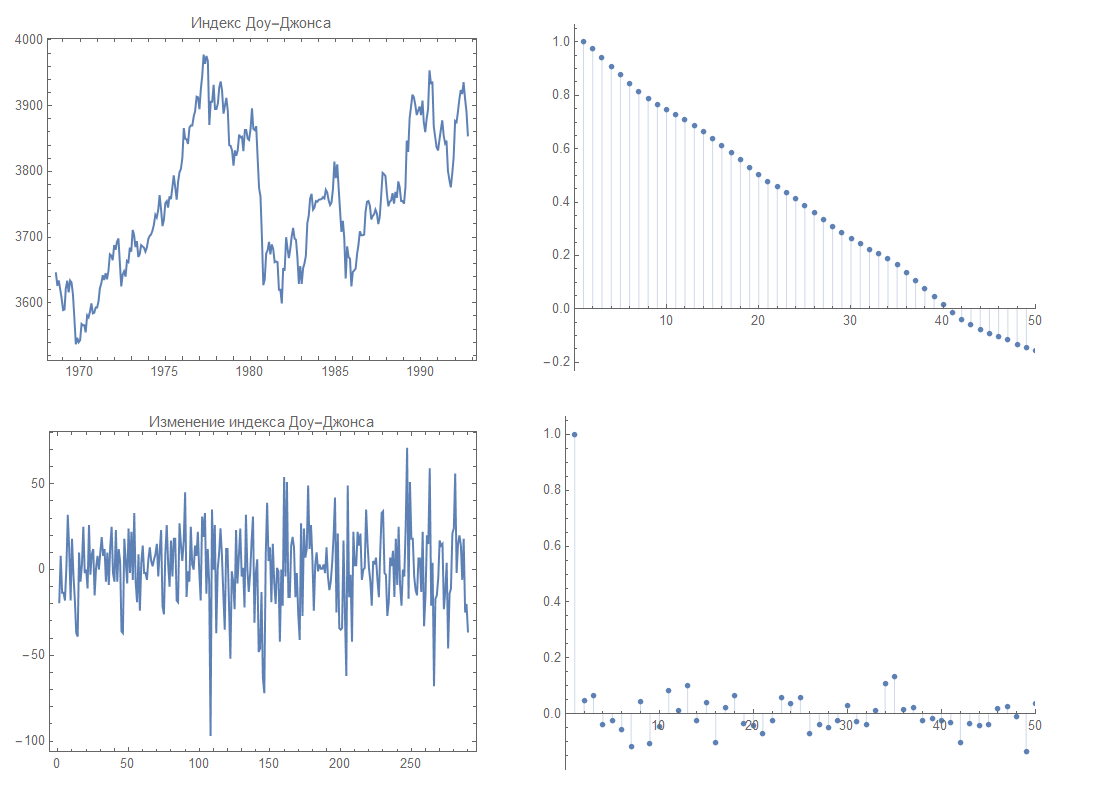
\includegraphics[scale=0.37]{images/4.png}
	Рис. 5: Вверху - нестационарный ряд, имеется ярко выраженный тренд, внизу - стационарный после сезонного дифференцирования
\end{center}

\textbf{Обратное преобразование}

Исходя из правил дифференцирования, перевод к исходному временному ряду может быть получен по следующему правилу:
$$y_t' = y_t - y_{t-k} \Leftrightarrow y_t = y_t'+y_{t-k}$$
где $y_t$ - исходный ряд, а $k$ - лаг диффернцирования.


\newpage
\section{Наивные методы прогнозирования}

\subsection{Прогноз средним (Simple Average)}

Наиболее простой способ построить прогноз на $h$ точек вперед - посмотреть, какие значения име предшествовали и в качестве прогноза взять среднее значение по всему имеющемуся временному ряду:
$$\hat{y}_{T+h} = \frac{1}{T} \sum\limits_{t=1}^T y_t$$

Такой способ позволет получить прогноз на сколь угодно длительный период времени и в задачах, где нет явных закономерностей во временном ряду, наивный прогноз средним значением является не худшим вариантом.

Недостатки прогноза средним: если в данных наблюдается \textit{тренд}, то среднее значение плохо описывает динамику поведения ряда, очень плохо..

\begin{center}
	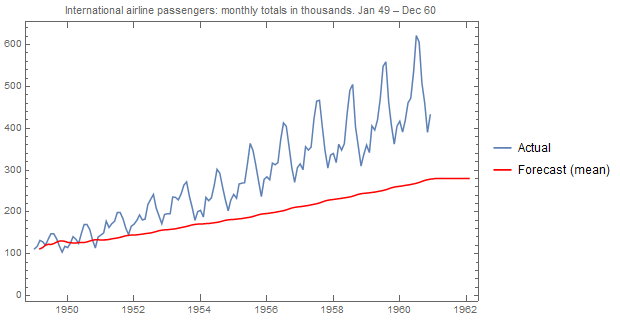
\includegraphics[scale=0.5]{images/6.png}

	Рис. 6 Прогнозирование средним, прогнозируется плохо в рядах с трендом
\end{center}

Видно, что прогноз сильно остает от тренда из-за того, что в начале ряда значения малые и перетягивают прогноз на себя.

Попытаемся улучшить метод прогнозирования для учитывания тренда.

\newpage
\subsection{Скользящее среднее (Moving Average)}

Чтобы сгладить недостатки предыдущего метода прибегают к методу \textit{скользящего среднего}. Прогноз будущего значения признака зависит от среднего по $k$ последних наблюдений, где $k$ - \textit{ширина окна}:
$$\hat{y}_{T+h} = \frac{1}{k} \sum\limits_{t = T-k+1}^T y_t$$

Само же сглаживание исходного ряда может быть записано следующим образом:
$$\hat{y}_i = \frac{1}{k} \sum\limits_{l=i}^{i+k-1} y_l$$

Действительно, допустим, что у нас есть ряд $y_i = [1.5,2.0,2.5,3.0,3.5,4.0], i = 1,\ldots,6$. Зададим ширину обзора нашего ряда: $k=3$. Выполненися сглаживания скользящим средним происходит следующим образом, как показано на рисунке:

\begin{center}
	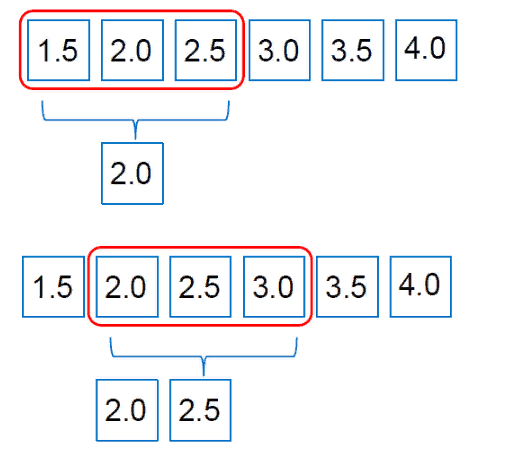
\includegraphics[scale=0.37]{images/7.png}

	Рис. 7 Принцип работы скользяшего среднего для ширины окна $k=3$
\end{center}

Для данного ряда прогноз на $1$ день вперед будет равен:
$$y_7 = \frac{3.0+3.5+4.0}{3} = 3.5$$

Долгосрочный прогноз таким способом построить не удастся, поскольку каждое следующее значение зависит от фактически наблюдаемых величин. Однако скользящее среднее позволяет сгладить исходный ряд, выявив таким образом тренд и предоставляя возможность обнаружить закономерности в данных.

При применении метода меньших порядков становятся более очевидными сезонные колебания. 

В общем, мы видим, что данная техника извлекает основные структуры из временных рядов. Но для лелинейной структуры тренда, например, скользящее среднее будет оставать от тренда и это становится более серьезной проблемой.

Значит, можно рассмотреть модифицированный способ сглаживания
\subsubsection{Взвешенное скользящее среднее (Weighted Moving Average)}

Вместо того, чтоы присваивать одинаковые веса всем наблюдениям, присвоем веса экспоненциально. Существует много способов генерации весов. Один из них:
$$\sum\limits_{i=1}^k w_{t-i}^k = 1$$
где $k$ - ширина обзора нашего ряда. Мы видим, что каждому значению присваивается определенный вес, причем значению, стоящему ближе к значению временного ряда, дается больший вес.

Веса можно раздавать и другими способами, тогда модель будет называться просто - \textit{взвешенное скользящее среднее}.


\newpage
\subsection{Наивный прогноз}

Еще более простой метод краткосрочного прогнозирования основан на предположении, что будущие значения переменной зависят от последнего наблюдаемого значения:
$$\hat{y}_{T+h} = y_T$$

Преимущество данного подхода - в простоте реализации и в отсутствии необходимости в большом количестве исторических данных. Недостаток - низкое качество прогнозирования.

Если развить идею, то в качестве прогноза можно брать предыдущие значения с сезонным лагом, если в данных наблюдается сезонность:
$$\hat{y}_{T+h} = y_{T+h-kS}, \qquad k = \left \lfloor \frac{(h-1)}{S} \right\rfloor + 1$$
где $S$ - период сезонности, а $\left \lfloor \_ \right \rfloor$ - частное от деления

\newpage
\subsection{Экстраполяция тренда}

При наличии во временном ряду тренда, можно усложнить наивную модель с помощью экстраполяции тренда:
$$\hat{y}_{T+h} = y_T + h \cdot \frac{y_T-y_1}{T-1}$$

Второе слагаемоме - уравнение прямой через две заданные точки, а именно через первую и последнюю точку заданного временного ряда. Таким образом можно построить долгосрочный прогноз, однако представленная модель не учитывает сезонные колебания.

\begin{center}
	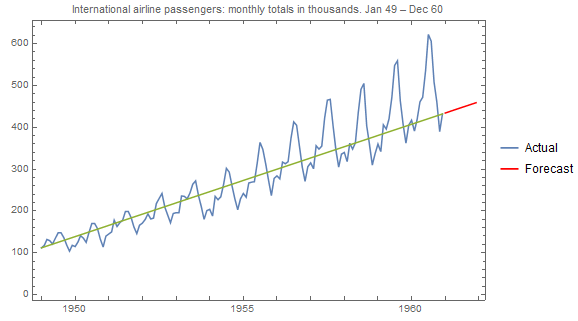
\includegraphics[scale=0.5]{images/8.png}

	Рис. 8 Экстраполяция тренда
\end{center}

\newpage
\section{Адаптивные методы краткосрочного прогнозирования}

\subsection{Простое экспоненциальное сглаживание (Модель Брауна)}

Экспоненциальнео сглаживание использует идею метода скользящего среднего с той лишь разницей, что каждое предшествующее наблюдение имеет свой вес, экспоненциально убывающий по мере углубления в историю.
$$\hat{y}_{T+1|T} = \alpha y_T + \alpha(1-\alpha)y_{T-1} + \alpha(1-\alpha)^2y_{T-2} + \ldots$$
где $\alpha \in [0;1]$ - коэффициент варьирования горизонта прошлого (smoothing constant, параметр сглаживания).

Вообще почему экспоненциальное сглаживание наывается экспоненциальным сглаживаением?) Разберем следующее доказательство:
\begin{proof}
	Запишем формулу члена $y_{t+1}$:
	$$y_{T+1} = \alpha y_T + (1-\alpha)y_{T-1}$$
	теперь запишем формулу для $y_{T}$:
	$$y_{T} = \alpha y_{T-1} + (1-\alpha)y_{T-2}$$
	Подставим $y_T$ в первую формулу:
	$$y_{T+1} =  \alpha(\alpha y_{T-1} + (1-\alpha)y_{T-2}) + (1-\alpha)y_{T-1}$$

	Мы видим, что $y_{T+1}$ зависит от $y_{t-1}$ как $\alpha^2$, если раскрыть скобки. Если мы будем дальше разворачивать, то на каждом шаге сам на себя умножается коэффициент. Любое наблюдение имеет экспоненциально малый вклад, потому что на каждом шаге убывает в $1-\alpha$ раз. Поэтому данный метод и называется методом экспоненциального сглаживания.
\end{proof}

Экспоненциальное сглаживание по данному методу также называют \textit{методом Брауна экспоненциального сглаживания}.

Экспоненциальное сглаживание учитывает, какое окно учитывают наблюдения. Чем больше параметр сглаживания $\alpha$, тем больший вес имеют последние наблюдения, тем больше они влияют на будущее предсказание. Поэтому $\alpha$ и называется \textit{коэффициетом варьирования горизонта прошлого.}

Модлеь экспоненциального сглаживания можно выразить через рекуррентную формулу:
$$\hat{y_{t+1|t}} = l_t, \qquad l_t = \alpha y_t + (1-\alpha)l_{t-1}$$
где $l_t$ - это сглаженное значения ряда на момент времени $t$, значение уровня ряда.

Таким образом, прогноз на один шаг вперед можно записать в виде:
$$\hat{y}_{T+1|T} = \left(\sum\limits_{i=0}^{T-1} \alpha(1-\alpha)^i \cdot y_{T-i} \right) + (1-\alpha)^T \cdot l_0$$

Данный метод подходит для \textit{краткосрочного прогнозирования} рядов \textit{без тренда и сезонности}. В качестве $l_0$ можно использовать арифметическую среднюю всех имеющихся данных или какой-то их части. Также можно взять в качестве $l_0$ первое значение временного ряда $y_1$.

Выбор оптимального значения $\alpha$ происходит таким образом, чтобы минимизировать среднюю квадратичную ошибку.

\newpage

\subsection{Метод Хольта}

\subsubsection{Метод Хольта с аддитивным трендом}

У экспоненциального сглаживания были недостатки - при прогнозе на долгосрочный срок метод эскпоненциального сглаживания предсказывал постоянное значение, не учитыва ни тренд, ни сезонность.

Учесть тренд позволяет \textbf{метод Хольта}, который предполагает разбиение временного ряда на две составляющие: уровень $l_t$ и тренд $b_t$. Экспоненциальное сглаживание применяется также к тренду в предположении, что будущее направление изменения ряда зависит от взвешенных предыдущих изменений. 

В случае линейного тренда:
$$\hat{y}_{t+h|t} = l_t + h \cdot b_t$$
$$l_t = \alpha y_t + (1-\alpha)(l_{t-1}+b_{t-1})$$ 
$$b_t = \beta(l_t-l_{t-1}) + (1-\beta)b_{t-1}$$
где $\alpha,\beta \in [0;1]$

Теперь компонента, описывающая уровень, зависит от текущего значения ряда, а второе слагаемое разбивается на предыдущее значение уровня и тренда.

Компонента, отвечающая за тренд, зависит от изменения уровня на текущем шаге и от предыдущего значения тренда. Результирующее значение прогноза - сумма модельных значений уровня и тренда. 

Данный метод также называют методом \textit{двойного экспоненциального сглаживания}. В качестве начального значения тренда можно брать разность между вторым и первым значением, что логично.

\subsubsection{Метод Хольта с мультипликативным трендом}

В случае мультипликативного тренда с затуханием
$$\hat{y}_{t+h|t} = l_t \cdot b_t^h$$
$$l_t = \alpha y_t + (1-\alpha)(l_{t-1} \cdot b_{t-1}^{\varphi})$$ 
$$b_t = \beta\left(\frac{l_t}{l_{t-1}}\right) + (1-\beta)b_{t-1}^{\varphi}$$
где $\alpha,\beta \in [0;1]$ и $\varphi \in [0,1]$ - параметр затухания.

Чтобы использовать обычный мультипликативный тренд, просто уберем коэффициент затухания.

\newpage
\subsection{Метод Хольта - Уинтерса}

В модели Хольта-Уинтерса возможны два подхода в зависимости от характера поведения сезонной составляющей. Рассмотренный ранее аддитивный метод применяется, когда сезонные колебания примерно постоянны по всему ряду.

\subsubsection{Метод Хольта - Уинтерса с аддитивной сезонностью}

Модель Хольта-Уинтерса является модификацией модели Хольта. Данная модификация позволяет учесть не только последние наблюдаемые значения и тренд, но и сезонность. Дополнительная сезонная компонента в модели объясняет повторяющиеся колебания вокруг уровня и тренда и характеризуется длиной сезона $m$:

Для реализации метода Хольта-Уинтерса с аддитивной сезонностью возьмем за основу реализацию метода Хольта и добавим сезонную составляющую:
$$\hat{y}_{t+h\, |\, t}=l_t+h\, b_t+s_{t-m+(h\bmod m)}\, ,$$
$$l_t=\alpha\, (y_t-s_{t-m})+(1-\alpha)\, (l_{t-1}+b_{t-1}),$$
$$b_t=\beta\, (l_t-l_{t-1})+(1-\beta)\, b_{t-1},$$
$$s_t=\gamma\, (y_t-l_{t-1}-b_{t-1})+(1-\gamma)\, s_{t-m}\, .$$

Уровень теперь зависит от текущего значения ряда без учета соответствующей сезонной компоненты, а сезонная компонента зависит от текущего значения ряда за вычетом уровня и от предыдущего значения компоненты.

\subsubsection{Метод Хольта - Уинтерса с мультипликативной сезонностью}

В случае, когда сезонные колебания изменяются пропорционально уровню ряда, говорят о мультипликативной сезонности. В данном случае мультипликативный метод Хольта-Уинтерса является предпочительным:
$$\hat{y}_{t+h\, |\, t}=(l_t+hb_t)\, s_{t-m+(h\bmod m )}\, ,$$
$$l_t=\alpha\, \frac{y_t}{s_{t-m}}+(1-\alpha)\, (l_{t-1}+b_{t-1}),$$
$$b_t=\beta\, (l_t-l_{t-1})+(1-\beta)\, b_{t-1},$$
$$s_t=\gamma\, \frac{y_t}{l_{t-1}+b_{t-1}}+(1-\gamma)\, s_{t-m}\, .$$

При аддитивном методе сезонная компонента $s_t$ выражается в абсолютных величинах в масштабе наблюдаемого ряда, а в уравнении уровня ряд сезонно корректируется путем вычитания из него сезонной компоненты. При использовании же мультипликативного метода сезонная компонента выражается в относительных единицах, а ряд корректируется путем деления значений на сезонную компоненту.

Метод Хольта-Уинтерса также часто называется \textit{тройным экспоненциальным сглаживанием} из-за сглаживания компонент уровня, тренда и сезонной составляющей.

\newpage

\section{Авторегрессионные методы прогнозирования}

\subsection{Модель авторегрессии AR}

\begin{definition}
	\textbf{Авторегрессия} порядка $p$ (AR(p)) - регрессия для ряда на его собственные значения в прошлом:
	$$y_t = \alpha + \alpha_1y_{t-1} + \alpha_2 y_{t-2} + \ldots + \alpha_py_{t-p} + \varepsilon_t$$
	$$y_t = \alpha + \sum\limits_{i=1}^p \alpha_p\cdot y_{t-i} + \varepsilon_t$$
	где $y_t$ - стационарный ряд, $\varepsilon_t$ - гауссов белый шум с нулевым средним и постоянной дисперсией.
\end{definition}

$y_t$ в данной модели представляет собой линейную комбинацию $p$ предыдущих значений ряда и шумовой компоненты.

\newpage
\subsection{Скользящее среднее MA}

Сразу отметим, что это не то, что мы разбирали раньше, то есть не простое, не взвешенное, не экспоненциальное скользящее среднее.

Будем считать, что будущее значение переменной зависит от среднего ее предыдущих значений. Это приводит к идее модели \textbf{скользящего среднего}:
$$y_t = \alpha + \varepsilon_t + \theta_1\varepsilon_{t-1} + \ldots + \theta_q\varepsilon_{t-q}$$
где $\varepsilon_t, \varepsilon_{t-1},\ldots,\varepsilon_{t-q}$ - значения шума в $q$ предыдущих моментах времени, $\alpha,\theta_1,\ldots,\theta_q$ - параметры модели, которые необходимо оценить. Эта модель называется моделью скользящего среднего порядка $q$ - MA(q).

\newpage
\subsection{ARMA}

Чтобы улучшить результаты предсказания модели, построим модель скользящего среднего на остатках, полученных после вычитания из исходных данных значений, предсказанных при помощи модели AP(p) $\varepsilon_i = y_i - \hat{y}_i$

\begin{definition}
	\textbf{Модель ARMA} - сумма авторегрессионной модели порядка p AR(p) и модели скользящего среднего порядка $q$ MA(q):
	$$y_t = \alpha + \sum\limits_{i=1}^p \alpha_i\cdot y_{t-i} + \varepsilon_t +  \theta_1\varepsilon_{t-1} + \ldots + \theta_q\varepsilon_{t-q}$$
\end{definition}

\begin{theorem}
	\textbf{Теорема Вольда} 

	Любой стационарный ряд может быт описан моделью ARMA(p,q) с любой точностью.
\end{theorem}

\newpage
\subsection{ARIMA}

В основе моделей класс ARIMA лежат идеи о том, что нестационарный ряд можно сделать стационарным при помощи дифференцирования, а любой стационарный ряд может быть описан моделью ARMA(p,q).

\begin{definition}
	ARIMA(p,d,q) - это модель авторегресии интегрированного скользящего среднего - модель ARMA(p,q) для $d$ раз продифференцируемого ряда.
\end{definition}

\newpage
\subsection{Тест Дики-Фуллера на стационарность}

Нестационарный временной ряд описывается моделью авторегресии интегрированного скользящего среднего ARIMA(p,d,q), если временной ряд $y_t$ является интегрированным порядка $d, d \geq 1$, а случайный процесс $\Delta^d y_t$ является стационарным и описывается моделью ARMA(p,q).

Рассмотрим модель авторегрессии первого порядка $AR(1)$:
$$y_t = \alpha + \alpha_1y_{t-1} + \varepsilon_1$$

Временной ряд $y_t$ является стационарным при $0 < \alpha_1 < 1$ и нестационарным интегрированным процессом при $\alpha_1= 1$. Во втором случае модель можно записать в следующем виде:
$$y_t = \alpha + y_{t-1} + \varepsilon_t$$

Такая модель называется \textbf{моделью случайного блуждания} или моделью единичного корня. Таким образом, значения параметра $\alpha_1$ влияет на тип модели временного ряда:

\begin{itemize}
	\item Если $\alpha_1 = 1$, то временной ряд нестационарный и описывается моделью случайного блуждания
	\item Если $\alpha_1 < 1$, то временной ряд стационарный и описывается моделью $AR(1)$.
\end{itemize}

В первом случае будущие значения рассматриваего ряда непредсказуемы, а во втором возникает возможность прогнозирования. Для финансово-экономических процессов значение $|\alpha_1| >1$ не свойственно, так как в этом случае процесс является взрывным

\textbf{Процесс проверки гипотезы теста Дики-Фуллера}

Тест Дики-Фуллера проверяет нулевую гипотезу, что ряд является \textit{нестационарным} и описывается моделью единичного корня при альтернативе $H_1$, что ряд является \textit{стационарным.} Проще говоря, для модели $AR(1)$ гипотезы принимают вид:
$$\begin{cases}
	H_0: \alpha_1 = 1  - \text{нестационарный ряд} \\
	H_1: \alpha_1 < 1 - \text{стационарный ряд}
\end{cases}$$

Процедура тестирования включает оценивание параметров модели $AR(1)$ с помощью МНК и проверку гипотез о значимости коэффициентов модели. Далее рассматриваются пороговые значения $t$-статистики Дики-Фуллера относительно коэффициента $\alpha_1$, которые представлены в виде таблиц для различных уровней значимости и различных значений длины ряда.

В качестве проверки гипотезы о нестационарности ряда, используется функция $statsmodels.tsa.stattools.adfuller$, возвращающее $pvalue$ для оцениваемого ряда. Если pvalue $ < T_{0.05}$, то нулевая гипотеза отвергается и ряд является стационарным. Однако важно, чтобы $pvalue$ был очень и очень маленьки, чтобы с большей степенью уверенности утверждать, что ряд является стационарным. 

Даже если тест Дики-Фуллера дал $pvalue$, для которого ряд стационарен, лучше проверить данную гипотезу еще раз теми метода, что были получены ранее.

\newpage
\subsection{SARIMA}

Пусть ряд имеет сезонный период длины $S$. Возьмем $ARMA(p,q)$:
$$y_t = \alpha + \sum\limits_{i=1}^p \alpha_i y_{t-i} + \varepsilon_t  + \sum\limits_{j=1}^q \theta_j \varepsilon_{t-j}$$
и добавим $P$ сезонных авторегрессионных компонент и $Q$ компонент скользящего среднего:
$$y_t = \alpha + \sum\limits_{i=1}^p \alpha_i y_{t-i} + \varepsilon_t  + \sum\limits_{j=1}^q \theta_j \varepsilon_{t-j} + \sum\limits_{r=1}^P \alpha_{rS} \cdot y_{t-r \cdot S} + \sum\limits_{l=1}^Q \theta_{lS} \cdot \varepsilon_{t-l \cdot S}$$

Результат - это модель $SARMA(p,q) \times (P,Q)$.

Модель $SARIMA(p,d,q) \times (P,D,Q)$ - модель $SARMA(p,q) \times (P,Q)$ для ряда, к которому $d$ раз было применено обычное дифференцирование и $D$ раз - сезонное. Такую модель часто называют просто $ARIMA$: первая буква не пишется, но подразумевается, что сезонная компонента тоже может быть.

Параметры $d,D$ необходимо подобрать так, чтобы ряд стал стационарным. Дифференцировать нужно как можно меньше, потому что с увеличением дифференцирования растет дисперсия итогового прогноза.

\subsubsection{Частичная автокорреляция}

\begin{definition}
	\textit{Частичная автокорреляция} - это автокорреляция после снятия авторегрессии предыдущего порядка.  
\end{definition}

Для определения значения частичной автокорреляции с лагом $2$, например, необхоидмо построить авторегрессию порядка $1$$AR(1)$, вычесть эту авторегрессию из ряда и вычислить автокорреляцию на полученных остатках, то есть:
$$pacf(h) = \begin{cases}
	\rho(y_{t+h}, y_t), \qquad h=1 \\
	\rho(y_{t+h} - AR(t, h-1), y_t - AR(t+h, h-1)), \qquad h \geq 1
\end{cases}$$
где $AR(t,h-1)$ - авторегрессия следующего вида:
$$AR(t,h-1) = y_t^{h-1} = \alpha_1y_{t+1} + \alpha_2y_{t+2} + \ldots + \alpha_{h-1}y_{t+h-1}$$
$$AR(t+h,h-1) = y_{t+h}^{h-1} = \alpha_1y_{t+h+1} + \alpha_2y_{t+h+2} + \ldots + \alpha_{h-1}y_{t+1}$$

Частичная автокорреляция используется для нахождения периодичностей во временных рядах и для определени порядка авторегрессионной модели ряда, чем мы и займемся ниже.


\subsubsection{Определение начального порядка авторегрессии и скользящего среднего (гиперпараметров)}

\begin{definition}
	\textit{Гиперпараметрами модели называют те параметры, которые задаются пользователем}. Параметрами же называют подобранные путем минимизации функционала качества моделью коэффициенты.
\end{definition}

Для выбора порядка авторегрессии обращаются к частичной автокорреляции.

Для выбора порядка авторегрессии $p_0$ мы ищем номер последнего значимого лага перед незначимым, для выборка сезонного порядка авторегрессии $P_0$ мы определяем величину сезонности, а после ищем номер последнего значимого сезонного лага перед незначимым.

\begin{center}
	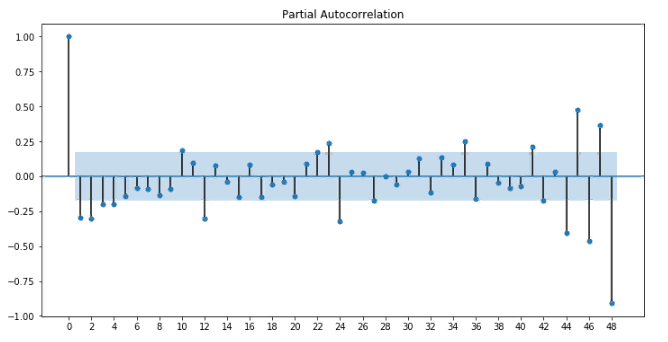
\includegraphics[scale=0.5]{images/9.png}

	Рис. 9 Определение начального порядка авторегрессии по частичной автокорреляции (PACF)
\end{center}

Так, в данном примере, последним значимый лаг оказался равным $4$, поэтому $p_0=4$. Период сезонности равен $12$, при лаге, равном $12$, частичная автокорреляци значима, при $24$ значима, а вот при $36$ уже нет. Следовательно, $P_0=2$. Теперь обратимся к определению порядка скользяшего среднего.

Для выборка порядка скользящего среднего обратимся к коррелограмме или автокорреляции.

Для начального значения $q_0$ выбираем последний значимый лаг перед следующим незначимым, для начального значения $Q_0$ определяем величину сезонности, а после выбираем последний значимый сезонный лаг перед следующим незначимым.

\begin{center}
	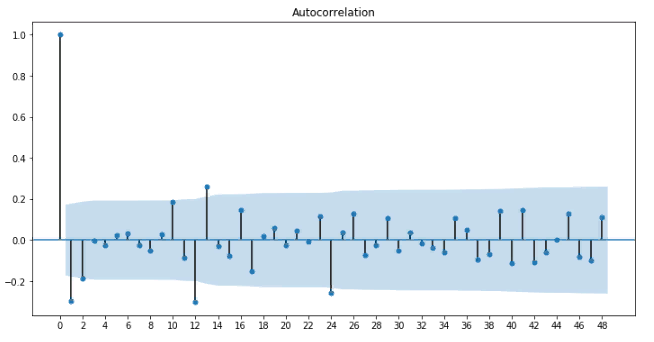
\includegraphics[scale=0.5]{images/10.png}

	Рис. 10 Определение начального порядка скользящего среднего по коррелограмме или автокорреляции (ACF)
\end{center}

Посдедний значимый лаг  - $2$. А последний значимый сезонный лаг равен $2$ (при лаге $12,24$ автокорреляция значима, при $36$ -  уже нет). Таким образом, $q_0=2, Q_0=2$.

Заметим, что гиперпараметры модели нельзя выбирать методом максимального правдоподобия, поскольку с увеличением количества парамтров значение функции правдоподобия $L$ растет.

Поэтому для сравнения различных моделей применяется информационный критерий Акаике:
$$AIC = 2K - 2\ln L$$
где $K=P + Q +p+q+1$ - число параметров в статистической модели, а $L$ - максимизированное значение функции правдоподобия модели.

Оптимальный по критерию Акаике будет модель с наименьшим значением этого критерия. Такая модель будет хорошо описывать даннные, а с другой - содержать не слишком большое количество параметров.

Параметры $p,P,q,Q$ определяются перебором и выбирается та комбинация, у которой Акаике меньший.

\newpage
\section{Методы оценки качества модели}

Чтобы оценить, насколько хорошо модель справляется с задачей прогнозирования, сравнить между собой различные модели или выбрать набор признаков, позволяющий налучшим образом описать данные, используются различные методы оценки сравнения качества.

\subsection{Отложенная выборка}

Для того чтобы оценка была достоверной, неправильно сравнивать качество модели на тех же данных, на которых она обучалась, то есть на которых были оценены параметры модели.  Очевидным способом оценки качества является разбиение всей выборки на две части: \textit{обучающую} (\textbf{train}) длины $l$ и \textit{контрольную} (\textbf{test}) длины $k$.

\begin{center}
	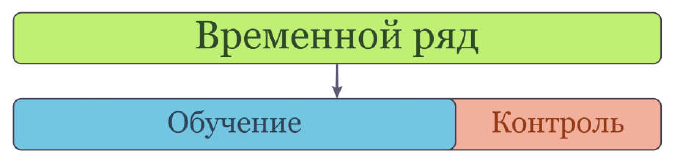
\includegraphics[scale=0.5]{images/11.png}

	Рис. 11 Разделение временного ряда на \textbf{train} и \textbf{test}
\end{center}

	
На тренировочном множестве модель обучается, а на \textit{тестовом} множестве происходит валидация результата. 

Данный метод логичен, но если разделить множество один раз на тестовое и тренировочное, то это может значительно повлиять на результат. Вдруг в тестовое множество случайно попали такие точки, в которых предсказать значение тяжелее или легче, чем обычно?

Тогда применяют следующий способ.
 
\newpage

\subsection{Перекрестная проверка (кросс-валидация) на временных рядах}

Давайте для сглаживания недостатков предыдущего метода применять так называемую \textbf{кросс-валидацию} (или перекрестную проверку) на временных рядах. Особенность задачи прогнозирования временных рядов состоит в том, что оценка качества модели может производиться только последовательно, так как временной ряд имеет временную структуру и порядок данных важен и перемешивать их нельзя.

\begin{center}
	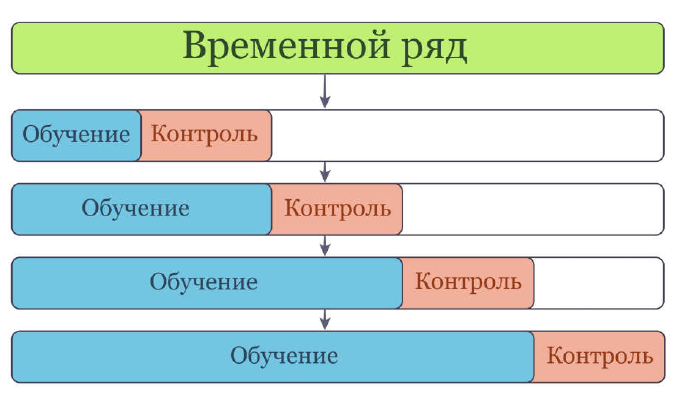
\includegraphics[scale=0.5]{images/12.png}

	Рис. 12 Кросс-валидация
\end{center}

Частным случаем метода кросс-валидации является контрольный по отдельным объектам (leave-one-out).

\newpage
\subsection{Метрики оценки качества}

\subsubsection{Коэффициент детерминации}

Цель регрессии - объяснение поведения $Y$. В любой выборке $Y$ оказывается низким, а в других - высоким. Разброс значений $Y$ можно описать с помощью суммы квадратов отклонений от выборочного среднего.
$$ \sum (Y - \overline{Y})^2 $$

Все показатели корреляции основаны на правиле сложения дисперсий $\Rightarrow$ можно разложить \textbf{общую сумму квадратов отклонений } переменной $Y$ от среднего значения $\overline{Y}$ на две части - \textbf{"объясненную" } сумму квадратов и \textbf{"необъясненную"}. 
$$\sum (Y - \overline{Y})^2 = \sum (\widehat{Y} - \overline{Y})^2 + \sum (Y - \widehat{Y})^2 \eqno (12)$$

Данное равенство можно переписать как:
$$SS_T = SS_R + SS_E \eqno (13)$$

где: 

$SS_T  = \sum (Y - \overline{Y})^2 $  - общая сумма квадратов отклонений \textit{(total sum of squares)}

$SS_R = \sum (\widehat{Y}-\overline{Y})^2 $ - \textbf{сумма квадратов отклонений, объясненная} регрессией, \textbf{факторная сумма} \textit{(sum of square due to regression)}

$SS_E = \sum (Y - \widehat{Y})^2  = \sum e_i^2 $ - \textbf{остаточная сумма} квадратов отклонений,
\textit{(sum of square due to error)}.

Введем \textbf{коэффициент детерминации}:
$$ R^2 = r^2 = \frac{\sigma_{y,obyasn}^2}{\sigma_{y,obch}^2} = \frac{SS_R}{SS_T} = 1 - \frac{SS_E}{SS_T} = 1 - \frac{\sum (Y - \widehat{Y})^2}{\sum (Y - \overline{Y})^2} $$
$$ R^2 = \frac{\sum (\widehat{Y}-\overline{Y})^2}{\sum (Y - \overline{Y})^2} = 1 - \frac{\sum (Y - \hat{Y})^2}{\sum (Y - \overline{Y})^2} $$

\textbf{Коэффициент детерминации}- обобщающий показатель оценки качества построенного уравнения регрессии.

Если фактор $x$ не влияет на результат, то линия регрессии параллельна оси ox  и $\bar{y} = \hat{y}$. Тогда вся дисперсия результативного признака обусловлена воздействием прочих факторов и общая сумма квадратов отклонений совпадет с остаточной.

Если же прочие факторы не влияют на результат, то $Y$ связан с $X$ функционально и остаточная сумма квадратов $SS_E = \sum e_i^2 = 0$. В этом случае сумма квадратов отклонений равна объясненной сумме квадратов: $$SS_T = SS_R$$

Поскольку не все точки поля корреляции лежат на линии регрессии, то всегда имеет место их разброс как обусловленный влиянием фактора $X$, т.е регрессией $Y$ по $X$, так и вызванный действием прочих причин(необъясненная вариация). 

Так как  $$ R^2 = 1 - \frac{\sum (Y - \widehat{Y})^2}{\sum (Y - \overline{Y})^2}  = 1 - \frac{SS_E}{SS_T},$$ 

то если $SS_T$ будет больше остаточной суммы квадратов $SS_E$, то уравнение регрессии статистически значимо и фактор $X$ оказывает существенное воздействие на результат $Y$. Это равносильно тому, что коэффициент детерминации $R^2$ будет приближаться к единице.

Числитель показывает дисперсию ошибки модели, а знаменатель – дисперсию рассматриваемого ряда. Таким образом, второе слагаемое показывает долю необъясненной моделью дисперсии ряда. 

Коэффициент детерминации принимает значения от $0$ до $1$. Чем ближе значение к $1$, тем
сильнее зависимость.

При расчете коэффициента множественной корреляции используется остаточная дисперсия, которая имеет систематическую ошибку в сторону преуменьшения, чем больше параметров определяется в модели при заданном объеме $n$, то есть его значение увеличивается с увеличением параметров модели, что не всегда является показателем того, что модель стала предсказывать лучше и обладает обобщающей способностью. Значение $R^2$ увеличивается от добавления в модель новых переменных, даже если эти переменные никакого отношения к объясняемой переменной не имеют. 

Поэтому принятно считать \textit{скорректированный} (нормированный) коэффициент множественной корреляции, учитывающий число степеней свободы, чтобы не допустить возможного преувеличения тесноты связи.
$$ R = \sqrt{1 - \frac{MS_E}{MS_T}}$$
$$ \hat{R^2} = 1 -(1-R^2) \frac{n-1}{n-m-1}$$
где $n$ - число наблюдений, а $m$ - число параметров.

Данный коэффициент зависит от объема наблюдения и числа параметров расчитываемой модели. Чем больше $m$, тем больше коэффициент детерминации и скорректированный коэффициент детерминации различаются.

Низкое значение скорректированного коэффициента детерминации означает, что в гегрессионную модель не включены существенные факторы, с другой стороны, рассматриваемая форма связи не отражает реальные соотношения между переменными, включенными в модель.

\subsubsection{Среднеквадратичная ошибка MSE}

В качестве метрики качества берут квадрат отклонения фактических значений от прогнозных (Mean Squared Error), которая выступает в качестве оптимизируемой функции при оценке параметров модели:
$$MSE = \frac{1}{T-k+1}\sum\limits_{t=k}^T (y_t - \hat{y}_t)^2$$

MSE достаточно удобная функция, ведь она выпуклая, дифференцируемая функция, но есть и недостатки - при больших значениях временного ряда MSE выдает большие значения, завышая их. Возможно и занижение ошибки, если $-1 \leq y \leq 1$.

\subsubsection{Средняя абсолютная ошибка MAE}

Наиболее интерпретируемой метрикой выступает средняя абсолютная ошибка (Mean Squared Error - MAE), которая показывает среднее отклонение прогнозных значений от фактических:
$$MAE = \frac{1}{T-k+1}\sum\limits_{t=k}^T |y_t - \hat{y_t}|$$

Недостатком данной метрики является невозможность сравнения качества, если решается задача прогнозирования нескольких временных рядов (разные величины имеют разные единицы измерения).

\subsubsection{Средняя абсолютная процентная ошибка}

Для сравнения качества для нескольких рядов можно сравнивать не абсолютную ошибку, а процентную (Mean Absolute Percentage Error):
$$MAPE = \frac{1}{T-k+1}\sum\limits_{t=k}^T \left|\frac{y_t - \hat{y}_t}{y_t}\right|$$

У MAPE есть недостаток - деление на ноль. И с этим нужно как-то жить и что-то придумывать. Некоторые программы отбрасывают периоды с нулевыми фактически значениями, но это не очень хорошая идея, потому что это фактически означает, что нам все равно, что мы прогнозировали, если значение нулевое.
\newpage

\subsubsection{Средняя симметричная абсолютная ошибка}

Идея симметричной абсолютной процентной ошибки: в знаменателе указать среднее между фактическим и прогнозным значениями:
$$SMAPE = \frac{1}{T-k+1} \sum\limits_{t=k}^T \frac{2|y_t - \hat{y}_t|}{|y_t|+|\hat{y}_t|}$$

\newpage

\section{Регрессионные модели прогнозирования}

\subsection{Понятие обучающей выборки. Предсказательная модель. Функция потерь и функционал качества}

\begin{definition}
	\textbf{Обучающая выборка} - набор пар $X^l = (x_i,y_i), i = 1,\ldots,l$, в котором для каждого объекта $x_i \in X^l$, характеризующегося рядом признаков $(x_{i1},x_{i2},\ldots,x_{im})$, известно значение целевой переменной $y_i$.
\end{definition}

\begin{definition}
	\textbf{Признаки} - числовые характеристики рассматриваемых объектов $X \to D_j, j = 1,\ldots, M$. В зависимости от принимаемых значений можно выделить следующие типы признаков:
\end{definition}

\begin{itemize}
	\item $D_j \in  \{0,1\}$ - бинарный
	\item $|D_j| < \infty$ - номинальный
	\item $|D_j| < \infty, D_j$ - упорядоченный порядковый
	\item $D_j \in R$ - количественный (вещественный)
\end{itemize}

Задача состоит в том, чтобы по обучающей выборке определить неизвестную зависимость $a: X \to Y$.

\begin{definition}
	\textbf{Предсказательная модель} - параметрическое семейство функций:
	$$A = \{a(x) = g(x,\theta) \, |\ , \theta \in \Theta\},$$
	где $gL X \times \Theta \to Y$ - фиксированная функция, а $\Theta$ - множество параметров модели.
\end{definition}

\begin{definition}
	$Q(a, X^l) $ называется \textbf{функционалом качества} алгоритма $a$ на обучающей выборке $X^l$. Величина ошибки накаждом объекте $x \in X^l$ называется \textbf{функцией потерь} $L(a,x)$:
	$$Q(a,X^l) = \frac{1}{l}\sum\limits_{i=1}^l L(a,x_i)$$
\end{definition}
\begin{definition}
	\textbf{Обучение модели} - процесс настройки параметров модели $\theta \in \Theta$ путем решения задачи оптимизации:
	$$Q(a, X^l) \to \underset{a \in A}{\min}$$
\end{definition}

\begin{definition}
	\textbf{Функция потерь} (Loss function) - это неотрицательная функция $L(a,x)$, характеризующая величину ошибки алгоиртма $a$ на объекте $x$.
\end{definition}

\subsection{Общий вид модели линейной регрессии. Предпосылки метода наименьших квадратов}

В соответствии с введенными ранее обозначениями, модель линейной регрессии может быть представлена в виде:
$$a(x) = g(x,\theta) = \theta_0 + \sum\limits_{j=1}^m \theta_j x_j$$
где $\theta_0$ - свободный член.

Если добавить фиктивный признак $x_0=1$ для каждого объекта, то модель линейной регрессии запишется так:
$$a(x) = g(x,\theta) = \sum\limits_{j=0}^m \theta_jx_j = (\theta, x) = \theta^Tx$$
где $\theta,x $ - вектора параметров коэффициентом и признаков. 

Таким образом, наблюдаемые значения $y$ описываются следующим выражением:
$$y = X \theta + \varepsilon$$
где $X$ - матрица "объекты-признаки", $\varepsilon$ - случайная непрогнозируемая ошибка.

\subsubsection{Предпосылки метода наименьших квадратов}

Условия, необходимые для получения несмещеных, состоятельных и эффективных оценок, представляют собой предпосылки МНК, соблюдение которых желательно для получения достоверности результатов.

Делаются предположения относительно поведения остатков $\xi_i$.

1. Модель линейна по параметрам

2. $\mathbb{E}\xi_i = 0 \forall i$, т.е ожидание значения случайного члена должно быть равно нулю в каждом наблюдении из-за того, что каждое наблюдение не должно включать в себя смещения ни в каком из направлений.

3. Гомоскедастичность - $\mathbb{D}\xi_i = Const $, т.е его значение в каждом наблюдении получено из распределения с постоянной теоретической дисперсией. Также не должно быть причин , делающих его больше подверженным ошибке в одних наблюдениях по сравнению с другим. Заметим, что $$\mathbb{E}\xi_i^2 = \mathbb{D}\xi_i = \mathbb{D}\sigma_{\xi_i}^2 | \forall i $$

4. Отсутствие автокорреляции остатков - значения случайного члена имеют взаимно независимые распределения. Случайный член не подвержен автокорреляции, т.е отсутствует систематическая связь между его значениями в любых двух наблюдениях.
Ковариация равна нулю:
$$ \sigma_{\xi_{i}\xi_{j}} = \mathbb{E}(\xi_i\xi_j) = \mathbb{E}\xi_i \cdot \mathbb{E}\xi_j = 0 | \forall i \neq j $$

5. $\xi_i \sim \mathbb{N}(0,\sigma^2)$: если случайный член нормально распределен, то распределены нормально и коэффициенты регрессии.

После построения уравнения регрессиии проводится проверка наличия у оценок $\xi_i$ тех свойств, которые предполагались. Связано это с тем, что оценки параметров регресии должны отвечать определенным критериям: быть несмещенными, состоятельными эффективными.

\begin{definition}
	Оценка является \textit{несмещенной}, если математическое ожидание остатков равно нулю.
\end{definition}

Следовательно, остатки не будут накапливаться и найденный параметр регрессии $b_i$ можно рассматривать как среднее значение из возможного большого количества несмещенных оценок.

\begin{definition}
	Оценки называются \textit{эффективными}, если они характеризуются наименьшей дисперсией.
\end{definition}

Это означает возможность перехода от точечного оценивания к интервальному.

\begin{definition}
	Состоятельность оценок характеризует увеличение их точности с увеличением объема выборки.
\end{definition}

При соблюдении введенных предпосылок, оценки, полученные методом наименьших квадратов, обладают данными важнейшими свойствами, на основании которых можно быть уверенным в достоверности результатов модели.

\begin{theorem}
	Теорема Гаусса-Маркова

	Пусть рассматривается модель линейной регрессии:
	$$y_i = X\theta + \varepsilon$$
	и выполнены предполсыки МНК. 

	Тогда оценки параметров $\theta_j$, полученные методом наименьших квадратов, будут \textbf{несмещенным и состоятельными}, а также оценка методов наимеших квадратов является \textit{оптимальной} в классе линейных несмешенных моделей.
\end{theorem}

\begin{proof}
	$\varepsilon_i = y_i - x_i \theta \sim N(0, \sigma^2)$, можно записать следующее:
	$$y_i \sim N(\theta^T\cdot x, \sigma^2)$$
	Тогда плотность нормального распределения выглядит следующим образом:
	$$f(y_i) = \frac{1}{\sqrt{2\pi}\sigma}e ^{-\frac{(y_i - \theta^T x_i)}{2\sigma^2}}$$
	Составим функцию правдоподобия:
	$$L =\prod\limits_{i=1}^n \frac{1}{\sqrt{2\pi}\sigma}e ^{-\frac{(y_i - \theta^T x_i)}{2\sigma^2}} \to \max$$

	Прологарифмируем:
	$$\ln L(\mu,\sigma) = \ln \left(\frac{1}{(\sqrt{2\pi}\cdot \sigma)^n}\right) + \left(-\frac{1}{2}\sum\limits_{i=1}^n \frac{(y_i - \theta^Tx_i)^2}{\sigma^2}\right) \to \max$$
	$$\sum\limits_{i=1}^n (y_i - \theta^T x_i)^2 \to \min$$

	А это и есть метод наименьших квадратов!
\end{proof}

\subsubsection{Применение модели линейной регрессии для прогнозирования}

Найдем решение МНК в общем виде. Запише выражение, которое надо минимизировать в матричной форме $L = (\theta X-y)^T(X\theta y) \to \min$, где $X$ - матрица объектов-признаков, а $\theta$-вектор искомых коэффициентов модели.

Продифференцируемым по всем переменным $\theta_k$ и приравняем производные к нулю:
$$\frac{\partial L}{\partial \theta} = \frac{\partial L}{\partial \theta}(\theta^TX^TX\theta - 2y^TX\theta + y^y)=0$$
$$2X^TX\theta = 2(y^TX)^T$$
$$\theta = (X^TX)^{-1}X^Ty$$
матрица $(X^TX)^{-1}X^T$ называется псевдообратной к матрице $X$. Это понятие является естественным обобщением понятия обратной матрицы на случай неквадратных матриц. 

Матрица $x$ выглядит следующим образом:
$$X = \begin{bmatrix}
	1 & x_{11} & x_{12} & \ldots & x_{1,m-1} \\
	1 & x_{21} & x_{22} & \ldots & x_{2,m-1} \\
	\ldots & \ldots & \ldots & \ldots \\
	1 & x_{n1} & x_{n2} & \ldots & x_{n,m-1} \\
\end{bmatrix}$$

На место элементов матрицы можно добавлять различные базисные функции, например, в качестве одного из столбцов добавить квадрат признака $x_1$, тогда мы будем строить квадратичную регрессию, то есть мы можем нагенерировать поведение признаков такое, какое захотим. Такой метод называется \textit{Feature Engineering}.

Подобным образом мы можем, например, использовать линейную регрессию для матрицы признаков, составленных из соответствующих гиперпараметрам сдвигам временного ряда.
\newpage
\subsection{Извлечение признаков из временного ряда. SARIMAX}

\subsubsection{Двойная сезонность}

Модель SARIMA позволяет строить прогнозные модели, учитывающие сезонность во временных рядах. Однако если сезонностей оказывается несколько, то возникает ряд проблем. Например, если имеется ряд дневных данных по спросу на товары, то могут наблюдаться одновременно, то возникает недельная, месячная и годовая сезонность.

В первую очередь нельзя нормально привести ряд к стационарному, ведь если проводить сезонное дифферцнирование, то для этого требуется определить длину сезонного лага, что не удастся сделать, если мы рассматриваем, например, високосный и невисокосный год $366$ и $365$ дней соответственно.

Более того, почему именно дата год назад учитывается в прогнозе? Ведь сегодня может быть будний день, а год назад мог быть выходной и спрос мог быть совершенно другим, а модель может этого не заметить.

Получается, что для описания поведения такого ряда необходимо выявить те характеристики, которые невозможно описать моделью SARIMA и строить модель с учетом особенностей ряда.

\subsubsection{Модель SARIMAX}

\begin{definition}
	Модель \textbf{SARIMAX} - расширение модели SARIMA, которая учитывает дополнительные факторы, которые помогают лучше описать поведение рассматриваемого временного ряда.
\end{definition}

Данную модель строят в два этапа:

\begin{enumerate}
	\item На первом шаге выделяют набор факторов $X$, которые характеризуют те зависимости в данных, которых не может учесть модель авторегрессии. Это могут быть как факторы, полученные непосредственно из временного ряда, так и сторонние, такие как погода, температура воздуха и.т.д.

	На полученном наборе факторов строят модель линейной регрессии:
	$$y_t = \sum\limits_{j=0}^m \theta_jx_{tj} + \varepsilon_t$$
	где $m$ - количество выделенных прогнозных факторов, $\varepsilon_t$ - непрогнозируемая ошибка модели. $x_{t0} =1$, так как необходимо учесть свободный член в модели.
\end{enumerate}

Затем находят остатки построенной модели и приближают их моделью SARIMA. Таким образом, если одна из сезонностей была учтена с помощью факторов на первом шаге, то вторую сезонность можно учесть в модели SARIMA.

\subsubsection{Извлечение факторов из временного ряда}

Если удачно определить набор факторов, описывающих поведение ряда, то остатки модели могут оказаться шумом. В качестве факторов могт выступать моменты времени, индикаторы для дня недели, статистики, посчитанные на данных из прошлого. Рассмотрим подробнее.

По сути, мы ищем способы, как добавить в матрицу признаков $X$ новые столбцы, чтобы модель оставляла в остатках как можно меньше информации.

\textbf{Зависимость от времени}

В качестве факторов, описывающих поведение ряда, можно использовать моменты времени $t$. Поскольку значения целевой переменной $y$ измеряются через равные промежутки времени, то наблюдаемая зависимость:
$$y_t = \sum\limits_{j=0}^m \theta_jt^j + \varepsilon_t$$

Таким образом, $m$ может быть степенью полинома, которым будет описана целевая переменная.

\textbf{Сезонные факторы}

Допустим, в остатках осталось много информации. Для улучшения качества модели посмотрим на сезонную составляющую. В качестве фактора можно использовать, например, индикатор текущего месяца. Первая запись получит $1$ - январь, $12$ - декабрь.

\begin{center}
	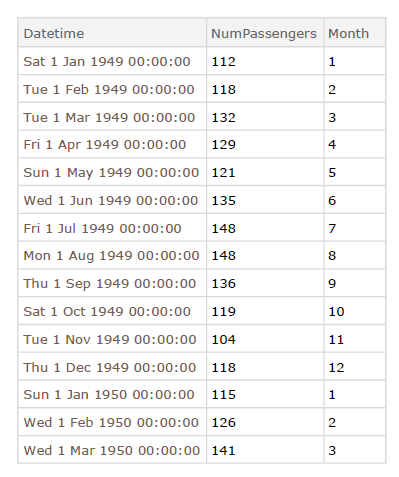
\includegraphics[scale=0.5]{images/13.png}

	Рис. 13 Сезонные факторы, нумерация месяцев
\end{center}

Также стоит не забывать о существовании праздников и каникул, будний день можно выделить $0$, а выходной - $1$. можно добавить и годовую, и недельную сезонность, если это важно. Необходимо также учитывать спефицику ряда, а именно учитывать предпраздничные дни и их динаминку, например. То есть необходимо тщательно продумать выбор факторов при добавлении сезонности.

\textbf{Тригонометрический ряд Фурье}

Хорошим способом описать сезонные колебания является применение Фурье-преобразований. Недостаток прошлого способа кодирования - расстояние от явнаря до декабря оказалось больше, чем от января до октября, что мешает выявить соответствующие закономерности. Решить данную задачу позволяет следующее преобразование:
$$\varphi_i = \sin \left(\frac{2\pi(i-1)}{s}\right), \psi_i = \cos \left(\frac{2\pi(i-1)}{s}\right)$$
где $i$ - соответствующее наблюдению значение  - месяц, например, отсчет ведем с нуля, а $s$ - длина сезонного колебания.

Дневная сезонность, состоящая из $24$ часов описывается следующим образом:

\begin{center}
	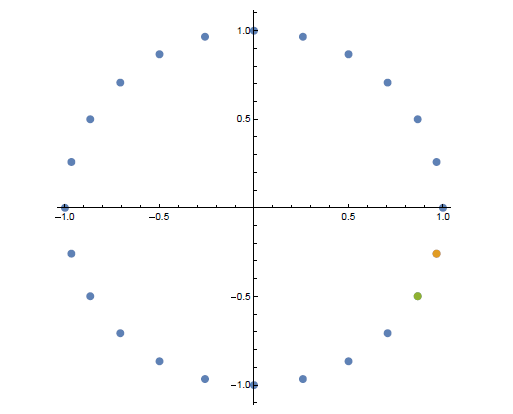
\includegraphics[scale=0.5]{images/14.png}

	Рис. 14 Дневная сезонность
\end{center}

Выделенные точки соответсттвуют значениям $0$ и $23$, а значит $0$ находится от $22$ на таком же расстоянии, как и от $2$, что соответствует реальной разнице во времени. Таким образом, значения $\varphi_i,\psi_i$ позволяют моделировать сезонные колебания с \textbf{постоянной амплитудой}, то есть для аддитивной сезонности. Добавим факторы в регрессионную модель, описываемую полиномом $m$ой степени и получим:
$$y_t = \sum\limits_{j=0}^m \theta_jt^j + \beta_1 \varphi_{t \operatorname{mod} s} + \beta_2 \psi_{t \operatorname{mod} s} + \varepsilon_t$$

Коэффициенты $\beta_1$ и $\beta_2$ находятся с помощью МНК.

На случай мультипликативной сезонности логично предположить, что с ростом ряда необходимо увеличиение амплитуды колебаний, поэтому домножим на $t$ или возведем в степень:
$$y_t = \sum\limits_{j=0}^m \theta_jt^j + \beta_1 \varphi_{t \operatorname{mod} s} \cdot t + \beta_2 \psi_{t \operatorname{mod} s} \cdot t+ \varepsilon_t$$

\textbf{Обработка категориальных переменных}

При решении практических задач возникает необходимость также кодировать
категориальные переменные. К категориальным переменным относятся, например,
город, в котором совершалась покупка или тип осадков, если для прогнозирования
используются погодные факторы. Можно закодировать все города, где есть торговые
точки сети через некоторые идентификаторы. Допустим, у нас есть точки в Москве,
Санкт-Петербурге и Сочи. Тогда:
$$\begin{cases}
	\text{Москва} \to 1 \\
	\text{Санкт-Петербург} \to 2 \\
	\text{Сочи} \to 3 \\
\end{cases}$$

Оказалось, что Сочи больше Москвы и такой способ кодирования не несет никакой информации. Можно отталкиваться от населения и присвоить номер больший самому большому городу.

Способ преобработки данных определяется из специфики задачи. Однако есть и универсальные методы.

Одним из них является \textbf{One-Hot-Encoding} или кодирование в унитарный код, который
каждому значению сопоставляет двоичный код фиксированной длины, содержащий
только одну 1 на позиции, соответствующей данному значению.

\begin{center}
	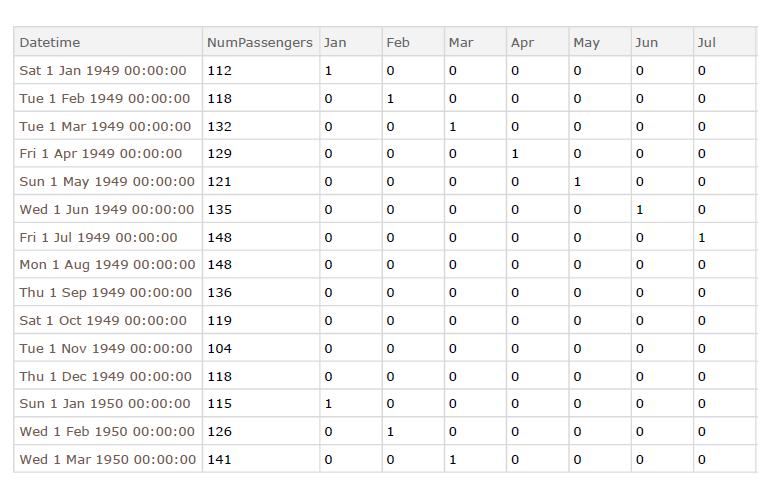
\includegraphics[scale=0.5]{images/15.png}

	Рис. 15 One-Hot-Encoding
\end{center}

При применение такого способа для описания всех $12$ месяцев достаточно $11$ колонок, иначе возникнет проблема мультиколлинеарности - зависимости признаков друг от друга.

Недостаток - хранение большой разряженной матрицы переменных. Другим способом является кодирование с помощью двоичного представления. Для $8$ значений - $3$ колонки, для $30$ - $5$ и.т.д.

Представленные способы хоть и продемонстрированы на примере кодирования, но они не решают проблему расстоний между месяцами.

\textbf{Дополнительная информация статистик}

Чтобы учесть отклонения от основных тенденций в качестве дополнительных факторов могут рассматриваться различные статистики, например:

\begin{itemize}
	\item средний показатель за тот же месяц в предыдущие годы
	\item среднеквадратичное отклонение показателя за тот же месяц в предыдущие годы
	\item отклонение показателей на прошлой неделе по сравнению с позапрошлой при прогнозировании на неделю вперед;
\end{itemize}

Таким образом, задача сводится к выявлению набора факторов (переменных,
признаков), наилучшим образом описывающих наблюдаемые закономерности.

\newpage
\subsection{Проблема переобучения. Регуляризация}

\subsubsection{Понятие недообучения и переобучения}

\begin{definition}
	\textbf{Недообучение} - называют нежелательное явление, когда алгоритм обучения не
обеспечивает достаточно малой величины средней ошибки на обучающей выборке.
Недообучение возникает при использовании недостаточно сложных моделей.
\end{definition}

\begin{definition}
	\textbf{Переобучение (overfitting)} - нежелательное явление, когда вероятность ошибки обученного алгоритма на объектах тестовой выборки оказывается существенно выше, чем средняя ошибка на обучающей выборке. Переобучение возникает при использовании избыточно сложных моделей.
\end{definition}

То есть, если мы используем достаточно сложную модель, например, многочлен высокой степени, у которой много параметров, то у модели появляется возможность выучить все точки, которые она видела.

Таким образом нужно следить, чтобы модель хорошо описывала данные, но при этом не слишком настраивалась под них.

\begin{definition}
	Говорят, что алгоритм обучения обладает \textbf{обобщающей способностью}, если вероятность ошибки на тестовой выборке достаточно мала или хотя бы предсказуема, то есть не сильно отличается от ошибки на обучающей выборке.
\end{definition}
\newpage

\subsubsection{Регуляризация}

Если используется слишком сложная модель, а данных недостаточно, чтобы точно
определить ее параметры, эта модель легко может получиться переобученной. Бороться
с этим можно различными способами:

\begin{itemize}
	\item взять больше данных (но, понятное дело, что такое не всегда доступно).
	\item упростить модель, исключи некоторые признаки, потому что модельможет быть на них заточена.
	\item использовать регуляризацию. У переобученной линейной модели значения параметров в модели становятся огромными и разными по знаку. Если ограничить значения весов модели, то с переобучением можно до какой-то степени бороться.
\end{itemize}

Рассмотрим методы регуляризации. Основнымиявляются $L_2$ - (\textit{ridge-регрессия} или гребневая регрессия) и добавление $L_1$-регуляризатора \textit{lasso-регрессия}.

\subsubsection{Гребневая регрессия}

Метод наименьших квадратов состоит в минимизации функционала качества:
$$Q(a,X^l) = \sum\limits_{i=1}^l \left(\sum\limits_{j=0}^m \theta_jx_{ij}-y_i\right)^2 \to \underset{\theta}{\min}$$

Большие значения параметров $\theta$ приводят к переобучению, добавим в функционал качества штраф на слишком большие значения $\theta$:
$$Q(a,X^l) = \sum\limits_{i=1}^l \left(\sum\limits_{j=0}^m \theta_jx_{ij}-y_i\right)^2 + \lambda \sum\limits_{j=1}^m \theta_j^2 \to \underset{\theta}{\min}$$

Такая модель называется гребневой регрессией.

\subsubsection{Лассо регрессия}

Отличие лассо-регрессии лишь в том, что штрафующим слагаемым выступает модуль:
$$Q(a,X^l) = \sum\limits_{i=1}^l \left(\sum\limits_{j=0}^m \theta_jx_{ij}-y_i\right)^2 + \lambda \sum\limits_{j=1}^m |\theta_j| \to \underset{\theta}{\min}$$

\subsubsection{Особенности регуляризаторов}

Рассмотрим особенности регуляризаторов

Пусть матрица "объекты-признаки" $X$ является единичной матрицей размера $l \times l$:
$$X = \begin{bmatrix}
	1 & 0 & \ldots & 0 \\
	0 & 1 & \ldots & 0 \\ 
	\ldots & \ldots & \ldots & \ldots \\ 
	0 & 0 & \ldots & 1 \\  
\end{bmatrix}$$

Тогда при решении задачи линейной регрессии использование МНК без регуляризации:
$$Q(a,X^l) = \sum\limits_{i=1}^l (\theta_i - y_i)^2 \to \underset{\theta}{\min}$$
дает следующий вектор $\theta$:
$$\theta_i^* = y_i$$

При добавлении $L_2$ регуляризации получаем:
$$\sum\limits_{i=1}^l (\theta_i - y_i)^2 + \lambda \sum\limits_{j=1}^l \theta_j^2 \to \min$$
$$2(\theta_i - y_i) + 2\lambda \theta_i = 0 $$
$$\theta_i = \frac{y_i}{1-\lambda}$$

А при добавлении $L_2$ регуляризации получаем:
$$\sum\limits_{i=1}^l (\theta_i - y_i)^2 + \lambda \sum\limits_{j=1}^l |\theta_j| \to \min$$

Если $\theta_i >0$, то $2(\theta_i - y_i) + \lambda = 0 \Longrightarrow \theta_i^* = y_i - \frac{\lambda}{2}$. 

Если $\theta_i < 0$, то $2(\theta_i - y_i)  -  \lambda = 0 \Longrightarrow \theta_i^* = y_i + \frac{\lambda}{2}$. 

Если $\theta_i = 0$, то $\theta_i^* = 0$:
$$\theta_i^* = \begin{cases}
	y_i - \frac{\lambda}{2}, \theta_i > 0 \\
	y_i + \frac{\lambda}{2}, \theta_i < 0 \\
	0, \theta_i = 0
\end{cases}$$

При использовании $L_2$-регуляризации зависимость $\theta_i^*$ от $y_i$ все еще линейная, компоненты вектора весов ближе расположены к нулю.

\begin{center}
	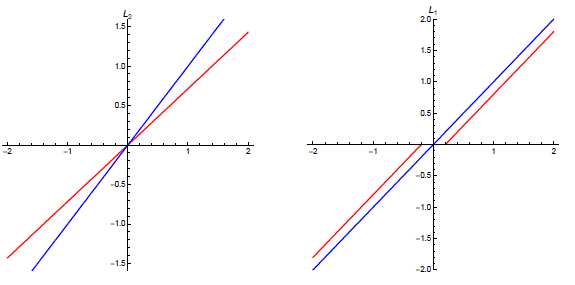
\includegraphics[scale=0.5]{images/16.png}

	Рис. 15 Регуляризация
\end{center}

В случае $L_1$-регуляризации график выглядит иначе: существует область размера $\lambda$ значений $y_i$, для которых $\theta_i = 0$. То есть $L_1$ позволяет отбирать признаки, а именно: параметры веса признаков, обладающих низкой предсказательной способностью, оказываются равными нулю.

\newpage
\section{Обобщенные линейные модели}

\subsection{Понятие функции связи. Роль функции связи в прогнозировании.}

Обобщенные линейные модели обеспечивают единый подход к моделированию всех типов целевых переменных. Рассмотрим общий вид линейной модели:
$$y = X\theta + \varepsilon$$

Введем следующее обозначение: $\eta = X\theta$ как часть линейного предиктора.

Обобщение линейных моделей происходит следующими способами:

\begin{itemize}
	\item В модели линейной регрессии делается предположение о том, что компоненты $y$ независимые нормально распределённые случайные величины с постоянной дисперсией. Мы можем расширить это предположение чтобы использовать любое распределение из тех, что принадлежат экспоненциальному семейству распределений: нормальное, пуассоновское, гамма и биномиальное.
	\item Вместо того, чтобы оценивать целевую переменную $\mu = E(y)$ как функцию линейного предиктора $X\theta$, ,будем оценивать некоторую функцию $g(\mu)$ от параметра $\mu$. Таким образом параметр распределения связан с линейной комбинацией следующей формулой:
	$$g(\mu) = \eta = X\theta$$
\end{itemize}

В обобщенных линейных моделях ожидаемые значения отклика представляют собой линейную комбинацию предикторов, которые связаны с зависимой переменной через функцию связи $g$:

Функция $g(\cdot)$ в формуле называется \textit{функцией связи}. 

\begin{definition}
	\textbf{Функция связи} - это функция, связывающая ожидаемое значение переменной $Y$ с предикторами $X_0,\ldots,X_m$. Функция $g(\cdot)$ должна быть монотонной и дифференцируемой, ведь для монотонной функции можно обратить функцию:
	$$g^{-1}(g(\mu)) = g^{-1}(X\theta) = \mu$$

	Выбор функции связи зависит от типа данных
\end{definition}

Функция связи используется в откликах модели, когда предполагается \textbf{нелинейная связь зависимой переменной с предикторами}.

Таким образом, спецификация обобщенной линейной модели включает в себя:

\begin{itemize}
	\item Выбор распределения
	\item Определение функции связи $g(\cdot)$
	\item Спецификацию линейного предиктора $X\theta$
\end{itemize}

\subsubsection{Оценка распределения целевой переменной}

Линейные модели крайне полезны для анализа данных. Тем не менее, линейные модели во многих отношениях являются ограниченными. Формально, классические приложения линейных моделей опираются на предположения о нормальности, линейности и гомоскедастичности.

Обобщение линейной модели, которое будет представлено в этой главе, позволит моделировать данные используя не только нормальное распределение.

В линейных моделях целевую переменную $Y$ чаще всего считают количественной, нормально распределенной величиной. Но это не единственный тип переменных, который встречается на практике. Вот некоторые примеры типов целевых переменных:

\begin{itemize}
	\item вещественные
	\item счетные
	\item бинарные
	\item переменные в форме пропорций
	\item переменные в форме долей
	\item упорядоченные
\end{itemize}

\subsubsection{Экспоненциальное семейство распределений. Экспоненциальное семейство распределений}

Экспоненциальнальное семейство является классом распределений, который включает в себя много известных нам прежде распределений в специальной форме. Общий вид экспоненциального семейства распределений будет выглядеть следующим образом:
$$f(y,\alpha,\varphi) = exp \left[\frac{y\cdot \alpha - c(\alpha)}{\varphi} + h(y,\varphi) \right]$$
где $h(\cdot)$ и $c(\cdot)$ - некоторые функции, а $\alpha$ называется \textit{каноническим параметров}, $\varphi$-параметр дисперсии.

Есть еще следующие выражение для статистик $\mu$:
$$Ey = \mu = c'(\alpha) \qquad  \qquad Dy = \varphi c''(\alpha)$$

Некоторые распределения являются частными случаями экспоненциального семейства распределений, которые мы будем получать в дальнейшем.

\newpage
\subsection{Функционал качества и функция связи в предположении нормального распределения целевой переменной.}

Обобщенные линейные модели расширяют модели линейной регрессии: предсказываемые значения связаны линейной комбинацией входных переменных через обратную функцию связи $g$:
$$\hat{y}(\theta,X) = g(\theta X)$$

Пусть случайная величина $y$ распределена по следующему закону:
$$y_i = \sum_{j=0}^m \theta_j x_{ij}+ N(0,\sigma^2) = N(\sum_{j=0}^m \theta_j x_{ij},\sigma^2)$$

То есть $$\mu  = \sum_{j=0}^m \theta_j x_{ij} = \left .\bar{\theta}\right .^T \cdot \bar{x}_i $$

Найдем оценку параметра $\theta$ методом максимального правдоподобия.

Функция правдоподобия записывается следующим образом:
$$L(\mu,\sigma) = \prod_{i=1}^n p(y_i,\mu,\sigma^2) = \frac{1}{(\sqrt{2\pi}\cdot \sigma)^n} \cdot e^{-\frac{1}{2}\sum\limits_{i=1}^n \frac{(y_i - \mu)^2}{\sigma^2}} \to \underset{\theta}{\max}$$

Прологарифмируем:
$$\ln L(\mu,\sigma) = \ln \left(\frac{1}{(\sqrt{2\pi}\cdot \sigma)^n}\right) + \left(-\frac{1}{2}\sum\limits_{i=1}^n \frac{(y_i - \mu)^2}{\sigma^2}\right)  =  \ln \left((\sqrt{2\pi}\cdot \sigma)^{-n}\right) -$$
$$ -\frac{1}{2}\sum\limits_{i=1}^n \frac{(y_i - \mu)^2}{\sigma^2}  = -n \ln \sqrt{2\pi\sigma^2} - \frac{1}{2\sigma^2}\sum\limits_{i=1}^n (y_i - \mu)^2  = $$
$$ = -\frac{n}{2} \ln (2\pi\sigma^2) -\frac{1}{2\sigma^2}\sum\limits_{i=1}^n (y_i -  \left .\bar{\theta}\right .^T \cdot \bar{x}_i)^2  \to \underset{\theta}{\max} $$
$$Q = - \frac{1}{2\sigma^2}\sum\limits_{i=1}^n (y_i -  \left .\bar{\theta}\right .^T \cdot \bar{x}_i)^2  \to \underset{\theta}{\max}$$

$Q$ является функционалом качества для нормального распределения.

В обобщенных линейных моделях ожидаемые значения отклика представляют
собой линейную комбинацию предикторов, которые связаны с зависимой переменной
через функцию связи g:
$$\mu = g^{-1}(\left .\bar{\theta}\right .^T \cdot \bar{x}_i)$$
$$g(\mu) = \left .\bar{\theta}\right .^T \cdot \bar{x}_i$$

Для нормального распределения, изначально было положено:
$$g(\mu) = \left .\bar{\theta}\right .^T \cdot \bar{x}_i = \mu$$

\textbf{Утверждение}: Нормальное распределение находится в классе экспоненциального семейства. Покажем это:
\begin{proof}
	$$f(y,\mu,\sigma^2) = \frac{1}{\sqrt{2\pi\sigma^2}} e^{-\frac{(y-\mu)^2}{2\sigma^2}} = exp \left[-\frac{y^2}{2\sigma^2}+\frac{y \mu}{\sigma^2} -\frac{\mu^2}{2\sigma^2} - \frac{1}{2} \log (2\pi \sigma^2)\right] = $$
	$$ = exp \left[ \frac{\mu y - \frac{\mu^2}{2}}{\sigma^2} - \frac{y^2}{2\sigma^2} - \frac{1}{2} \log (2\pi \sigma^2)\right]$$

	Это эксопненциальное распределение с:
	$$\alpha = \mu,  c(\alpha) = \frac{\alpha^2}{2}$$
	$$E(y) = \mu  = c' (\alpha)$$
	$$D(y) = \varphi \cdot c''(\alpha) = \sigma^2 \cdot 1 = \sigma^2 $$
	$$g(\mu)  =[c']^{-1}(\mu)$$
	$$c(\mu)' = \mu =\left .\bar{\theta}\right .^T \cdot \bar{x} $$

	Итого, для нормального распределения $N$:
	$$\left .\bar{\theta}\right .^T \cdot \bar{x} = g(\mu) \qquad g(\mu)=\mu \qquad \mu = g^{-1}(\left .\bar{\theta}\right .^T \cdot \bar{x})$$

	Данная функция связи называется \textit{тождественной функцией связи}.
\end{proof}

\newpage
\subsection{Прогнозирование счетной переменной}

Существуют задачи, где на $y$ наложены ограничения: например, $y$ должен быть целым и неотрицательным. В таком случае надо пользоваться не МНК, а другими способами. 

Если целевые переменные являются вещественными или счетными, а также если предположить, что $y$ неотрицательный, то можно использовать Пуассоновское распределение с логистической функцией связи, которую мы сейчас и получим.

Пусть величина $y \in \{0,1,2,\ldots, \}$, тогда для нее применимо распределение Пуассона:
$$y \sim Poiss(y=k, \lambda) = \frac{\lambda^k e^{-\lambda}}{k!}, \quad k =0, 1, 2,\ldots $$
$$Ey = \lambda, Dy = \lambda$$

Так как $\lambda $ должно быть больше нуля, то хотелось бы линейную комбинацию $(-\infty, \infty)$ переделать в промежуток $(0,\infty)$. Это можно сделать с помощью потенцирования.
$$\log y =  \left .\bar{\theta}\right .^T \cdot \bar{x} \Rightarrow \lambda = e^{\left .\bar{\theta}\right .^T \cdot \bar{x}}$$

Опять же найдем с помощью ммп логарифм функции правдоподобия
$$P(\xi = y)  = \frac{e^{-\lambda}\cdot \lambda^y}{y!}, y \in \{0,1,2,\ldots, \} $$
$$L(\lambda) = \prod\limits_{i=1}^n p(y_i,\lambda) = \prod\limits_{i=1}^n \frac{e^{-\lambda} \lambda^{y_i}}{y_i !}$$
$$\ln L(\lambda) = \sum\limits_{i=1}^n \ln \frac{e^{-\lambda} \lambda^{y_i}}{y_i !} =\sum\limits_{i=1}^n (-\lambda + y_i \ln \lambda - \ln(y_i !))$$

Последнее слагаемое не сожержит оцениваемого параметра $\lambda$, поэтому:
$$Q =\sum\limits_{i=1}^n (-\lambda + y_i \ln \lambda ) \to \underset{\theta}{\max}$$
$$Q = \sum\limits_{i=1}^n ( e^{\left .\bar{\theta}\right .^T \cdot \bar{x}}  - y_i \ln  e^{\left .\bar{\theta}\right .^T \cdot \bar{x}} ) \to \underset{\theta}{\min}$$
$$Q = \sum\limits_{i=1}^n ( e^{\left .\bar{\theta}\right .^T \cdot \bar{x}}  - y_i \bar{\theta}^T \cdot \bar{x} )\to \underset{\theta}{\min}$$

Для пуассоновского распределения:
$$g(\mu) = \log \lambda$$
$$\mu = g^{-1}(\log \mu) = e^{\log \mu} = \mu$$

\textbf{Утверждение}: Распределение Пуассона лежит в классе экспоненциального семейства, покажем это:
\begin{proof}
	$$f(y,\lambda) = exp\left(\frac{y\cdot\log\lambda - \lambda}{1} - log(y!)\right)$$
	$$\alpha = \log(\lambda), \lambda = exp(\alpha), c(\alpha) = \lambda, c(\lambda) = e^{\lambda}$$
	$$g(\lambda) = \log(\lambda) = \left .\bar{\theta}\right .^T \cdot \bar{x}$$

	И это верно, так как:
	$$\lambda = g^{-1}((g(\left .\bar{\theta}\right .^T \cdot \bar{x}))) = e^{\log \lambda} = \lambda$$

	Данная функция связи называется \textit{логистической функцией связи}.
\end{proof}

\newpage
\subsection{Прогнозирование времени наступления события. Анализ выживаемости}

Задача анализа выживаемости состоит в том, чтобы предсказать, сколько проживет человек, поступивший в больницу или в предсказании времени, которое пройдет до следующего события.

\textit{Экспоненциальное распределение} моделирует время между двумя последовательными свершениями одного и того же события и очень хорошо подходит для моделирования задачи анализа выживаемости.

Сначала покажем, что экспоненциальное распределение принадлежит экспоненциальному семейству распределения (было бы забавно, если бы не принадлежало):
\begin{proof}
$$f(y)=\mu e^{-\mu y} = \exp(-\mu y + \log \mu) = \exp \left( \frac{y(-\mu)+\log \mu}{1}- 0\right ) =  $$
$$ = \exp \left( \frac{y(-\mu)- (-\log \mu)}{1} - 0\right)$$
$$\alpha = -\mu \qquad c(\alpha) = -\log \mu$$
$$g(\mu) = \left .\bar{\theta}\right .^T \cdot \bar{x} = - \frac{1}{\mu}$$

И это верно, так как:
$$g^{-1} = \frac{-1}{\mu} \Leftrightarrow \mu = g^{-1}(g(\mu)) = -\frac{1}{\left(-\frac{1}{\mu}\right)} = \mu$$
\end{proof}

А теперь выведем функционал качества для задач анализа выживаемости используя метод максимального правдоподобия и функцию правдоподобия соответственно. Пусть $y$ подчиняется экспоненциальному распределению, которое является непрерывным:
$$P(y) = \mu e^{-\mu y}$$

В качестве функции связи возьмем следующую величину:
$$\lambda = -\frac{1}{\sum\limits_{j=0}^m \theta_j x_{ij}} = -\frac{1}{\left .\bar{\theta}\right .^T \cdot \bar{x}}$$

Запишем функцию правдоподобия:
$$L = \prod_{i=1}^n -\frac{1}{\left .\bar{\theta}\right .^T \cdot \bar{x}} \exp \left(\frac{y}{\left .\bar{\theta}\right .^T \cdot \bar{x}}\right) \to \max$$
$$\ln L = \sum\limits_{i=1}^n \ln\left(-\frac{1}{\left .\bar{\theta}\right .^T \cdot \bar{x}}\right) + \left(\frac{y}{\left .\bar{\theta}\right .^T \cdot \bar{x}}\right) \to \max$$ 
$$Q = \sum\limits_{i=1}^n \ln\left(-\left .\bar{\theta}\right .^T \cdot \bar{x}\right) - \left(\frac{y}{\left .\bar{\theta}\right .^T \cdot \bar{x}}\right) \to \min$$

Это и есть функционал качества для экспоненциального распределения, с помощью которого можно решать задачу анализа выживаемости.

Вкратце рассмотрим два распределения, также имеюищих важное значение.

\textit{Отрицательное биномиальное распределение} -  также называемое распределением Паскаля — это распределение дискретной случайной величины равной количеству произошедших неудач в последовательности испытаний Бернулли с вероятностью успеха $p$, проводимой до $n$-го успеха.
$$P(y=k) = C_{n+k-1}^k p^n(1-p)^k$$

\textit{Гамма распределение} широко применяется для моделирования сложных потоков событий, сумм временных интервалов между событиями, в экономике, теории массового обслуживания, в логистике, описывает продолжительность жизни в медицине. Является своеобразным аналогом дискретного отрицательного биномиального распределения.

Функция связи у гамма-распределения такая же, как у экспоненциального: $g(\mu) = \left .\bar{\theta}\right .^T \cdot \bar{x} = - \frac{1}{\mu}$. И гамма-распределение, и отрицательное биномиальное распределение входит в состав экспоненциального семества.


\newpage
\subsection{Применение биномиального распределения}

Биномиальное распределение - дискретное распределение вероятностей случайной величины $y$, принимающей целочисленные значения $k=0,1,\ldots,n$ и применяется для ситуаций, когда необходимо высчитать вероятность определенного количества усехов в последовательности из $n$ независимых экспериментов, таких, что вероятность успеха в каждом из них постоянна и равна $p$:
$$F(Y = y) = C_n^y \cdot p^y \cdot (1-p)^{n-y} \qquad Ey = np \qquad Dy = np(1-p)$$ 

Пусть $y \sim Bin(n,p)$. Запишем функцию вероятности и попытаемся вывести функцию связи для биномиального распределения:
$$F(Y = y) = C_n^y \cdot p^y \cdot (1-p)^{n-y} = \exp \left[\ln C_n^y + \ln p + (n-y) \ln (1-p)\right] = $$
$$ = \exp\left[y\ln\left(\frac{p}{1-p}\right) + n \ln (1-p) + \ln C_n^y \right]$$

В качестве $\alpha = \ln\left(\frac{p}{1-p}\right)$, то есть $p = \frac{e^{\alpha}}{1+e^{\alpha}}$, тогда подставив это в выражение, получим:
$$f(y,p) =\exp\left[y\cdot \alpha + n \ln \left(\frac{1}{1+e^{\alpha}}\right) + \ln C_n^y\right]$$

Биномиальное распределение содержится в экспоненциальном распределении со следующими параметрами:
$$\alpha = \ln\left(\frac{p}{1-p}\right) \qquad c(\alpha) = n \ln (1+e^{\alpha})$$

Соответственно функция связи имеет вид:
$$g(p) = \ln \frac{p}{1-p} = \left .\bar{\theta}\right .^T \cdot \bar{x} $$

Действительно, ведь:
$$p = g^{-1((g(p)))} = \frac{e^{g(p)}}{1+e^{g(p)}} = \frac{e^{\ln \frac{p}{1-p}}}{1+e^{\ln \frac{p}{1-p}}}  = p$$

Такая функция связи называется \textit{logit-функцией связи}.

Теперь с помощью метода максимального правдоподобия выведем функционал качества для биномиального распределения:
$$p = g^{-1((g(p)))} = \frac{e^{g(p)}}{1+e^{g(p)}} = \frac{e^{\left .\bar{\theta}\right .^T \cdot \bar{x}}}{1+e^{\left .\bar{\theta}\right .^T \cdot \bar{x}}}$$

Запишем функцию правдоподобия:
$$L = \prod\limits_{i=1}^l C_n^{y_i} p_i^{y_i}(1-p_i)^{n-y_i} \to\underset{\theta}{\max}$$
$$\ln L = \sum\limits_{i=1}^n \log C_n^{y_i} + y_i \log p_i + (n-y_i)\log(1-p_i) \to\underset{\theta}{\max}$$

Биномиальный коэффициент не содержит оцениваемого параметра $p$, поэтому функционалом качества биномиального распределения будет:
$$Q = \sum\limits_{i=1}^n y_i \log \frac{e^{\left .\bar{\theta}\right .^T \cdot \bar{x}}}{1+e^{\left .\bar{\theta}\right .^T \cdot \bar{x}}} + (n-y_i)\log(1-\frac{e^{\left .\bar{\theta}\right .^T \cdot \bar{x}}}{1+e^{\left .\bar{\theta}\right .^T \cdot \bar{x}}}) \to\underset{\theta}{\max}$$

\newpage
\subsection{GARMA}

GARMA переводится как Generalized Autoregressive Moving Average Models - модели скольязего среднего для обобщенных линейных моделей, у которых распределение целевой переменной не является нормальным гауссовским. Оценка модели выполняется с использованием итеративно взвешенного алгоритма наименьших квадратов.

Модели GARMA может быть исоплзована для распределения Пуассона, отрицательного биномиального распределения или для непрерывного $gamma$-распределения, называемое $GARCH$ моделью.

\subsubsection{Определение модели}

В GARMA моделе, условное распределение \textit{каждого наблюдения} $y_t, t = 1,\ldots,n$ вычисляется с учетом предыдущей информации
$$H_t = \{x_r,\ldots,x_1; \, y_{t-1},\ldots,y_1;\ ,\mu_{t-1},\ldots,\mu_1\}$$
в предположении о том, что данные наблюдения принадлежат одному и тому экспоненциальному семейству:
$$f(y_t | H_t) = exp \left[\frac{y_t \cdot \alpha - c(\alpha)}{\varphi} + h(y,\varphi) \right]$$
где $\alpha$ и $\varphi$ - канонический и параметр масштаба, $c(\cdot)$ и $h(\cdot)$ функции, определяющие экспоненциальное семейство функция и $x$, являющийся вектором из $r$ объясняющих переменных.

$$E(y_t|H_t) = \mu = c'(\alpha) \qquad  \qquad D(y_t|H_t) = \varphi c''(\alpha)$$
выражают условную вероятность каждого значения $y_t$ по $H_t$.

Как видно, обозначения здесь очень похожи на те, что и для независимых наблюдений GLM, но в данном случае моделируются условные распределения, что является важным уточнением модели.

Как и в стандартном GLM, параметр $\mu_t$ связан с предиктором $\eta_t$ с помощью дважды дифференцируемой мотонной функции $g$, которая называется \textit{функцией связи}.

По сравнению с GLM, где предиктор $\eta = \bar{x_t}^T \cdot \bar{\theta}$, где $\theta = (\theta_1,\theta_2,\ldots,\theta r)$, в данном случае добавляется компонента $\tau_t$, которая позволяет добавить автогресионную компоненту скользяшего среднего к предиктору. Прошлые значения, зависящие от вермени, также включены в предиктор.

Модель для $\mu_t$ в GARMA $g(\mu_t) = \eta_t = \bar{x_t}^T \cdot \bar{\theta} + \tau_t$ где:
$$\tau_t = \sum\limits_{i=1}^p \alpha_i y_{t-i} +  \sum\limits_{j=1}^q \theta_j \varepsilon_{t-j}$$
функции, которые представляют собой авторегрессионную $AR$ компоненту и компоненту скользящего среднего $MA$.

Данное выражение записывается по-другому:
$$g(\mu_t) = \eta_t = \bar{x_t}^T \cdot \bar{\theta} + \sum\limits_{i=1}^p \left(g(y_{t-i})-\bar{x}_{t-j}^T \cdot \bar{\theta}\right) +  \sum\limits_{j=1}^q \phi_j \left(g(y_{t-i})-\eta_{t-j}\right)$$

Данная модель в экспоненциальном семействе распределения называется моделью \textit{GARMA(p,q)}. Параметры $\theta, \alpha$ и $\phi$ определяются с помощью метода максимального правдоподобия.

\subsubsection{Poisson Garma(p,q)}

В предположении, что $g$ является логистической функции связи $g(\lambda_t) = \log(\lambda_t)$:
$$\log(\lambda_t) = \bar{x_t}^T \cdot \bar{\theta} + \sum\limits_{i=1}^p \left(\log(y_{t-i}^*)-\bar{x}_{t-j}^T \cdot \bar{\theta}\right) +  \sum\limits_{j=1}^q \phi_j \left(\log(y_{t-i}^*)-\lambda_{t-j}\right) $$

Так как $\alpha_t = \log(\lambda_t) =  \bar{x_t}^T \cdot \bar{\theta}$, то:
$$\log(\lambda_t) = \alpha_t + \sum\limits_{i=1}^p \left(\log(y_{t-i}^*)-\alpha_{t-i}\right) +  \sum\limits_{j=1}^q \phi_j \left(\log(y_{t-i}^*)-\lambda_{t-j}\right) $$

\newpage
\section{Дополнительные главы}

Мы обучались на многих библиотеках и многие функции мы использовали очень часто. Разберем некоторые из них.

Базовые библиотеки:

\begin{enumerate}
	\item \textbf{\textsc{import numpy as np}} - библиотека для ускоренных вычислений \textit{Numpy}
	\item \textbf{\textsc{import pandas as pd}} - для обработки данных \textit{Pandas}
	\item \textbf{\textsc{import matplotlib.pyplot as plt}} - для визуализации данных \textit{Matplotlib} 
	\item \textbf{\textsc{import seaborn as sns}} - библиотека \textit{Seaborn}, более качественная визуализация
\end{enumerate}

Документация \href{https://numpy.org/doc/stable/reference/}{Numpy}, 
\href{https://pandas.pydata.org/docs/}{Pandas}, 
\href{https://matplotlib.org/3.2.1/contents.html}{Matplotlib} и 
\href{https://seaborn.pydata.org/}{Seaborn}

\newpage
\subsection{Операции с временными рядами}

\begin{enumerate}
	\item \textbf{\textsc{scipy.stats.boxcox}} - преобразование Бокса-Коса, принимает временной ряд, в возвращает преобразованный ряд и значение $\lambda$, при котором достигается максимум правдоподобия
	\item \textbf{\textsc{scipy.stats.boxcox\_llf}} - возвращает значение функции правдоподобия
	\item \textbf{\textsc{pd.Series.diff(lag)}} - дифференцирование временного ряда с лагом $\tau$
	\item \textbf{\textsc{pd.Series.shift(n)}} - сдвиг на $n$ периодов ряда.
	\item \textbf{\textsc{from scipy.optimize import minimize}} - минимизация функции от параметра, параметр передается через $lambda$-функцию. 
\end{enumerate}

Документация \href{https://www.scipy.org/docs.html}{Scipy}

\newpage
\subsection{Statsmodels}

\begin{enumerate}
	\item \textbf{\textsc{import statsmodels.api as sm}} - вся библиотека \textit{Statsmodels} для прогнозирования временных рядов
	\item \textbf{\textsc{from statsmodels.tsa.holtwinters import}}
	\begin{enumerate}
		\item \textbf{\textsc{SimpleExpSmoothing}} - простое экспоненциальное сглаживание
		\item \textbf{\textsc{Holt}} - методы Хольта, двойное экспоненциальное сглаживание
		\item \textbf{\textsc{Exponential Smoothing}} - методы Хольта-Уинтерса, тройное экспоненциальное сглаживание
	\end{enumerate}
	\item \textbf{\textsc{from statsmodels.graphics.tsaplots import plot\_acf}} - коррелограмма, автокорреляционная функция (ACF)
	\item \textbf{\textsc{from statsmodels.graphics.tsaplots import plot\_pacf}} - график частичной автокорреляции (PACF)
	\item \textbf{\textsc{from statsmodels.tsa.arima\_model import ARIMA}} - построение модели ARIMA
	\item \textbf{\textsc{from statsmodels.tsa.statespace.sarimax import SARIMAX}} - модель SARIMA
	\item \textbf{\textsc{from statsmodels.tsa.stattools import adfuller}} - тест на стационарность Дики-Фуллера, возвращает pvalue вторым выходным аргументом
	\item \textbf{\textsc{from statsmodels.tsa.seasonal import seasonal\_decompose}} - разложение ряда на тренд, сезонную компоненту и случайную компоненту
\end{enumerate}

Документация \href{https://www.statsmodels.org/stable/examples/index.html}{Statsmodels}

\newpage
\subsection{Prophet}

Prophet для визуализации результатоп прогнозирования использует библиотеку \textbf{Plotly}, которая позволяет строить интерактивные графики.

Модель прогнозирования в библиотеке от Facebook имеет название \textbf{Prophet.} Основной идеей построения прогноза стало разложение временного ряда на основные составляющие:
$$y(t) = g(t) + s(t) + h(t) + \varepsilon_t$$
где $g(t)$ $-$ функция, описывающая тренд временного ряда, $s(t)$ $-$ компонента, описывающая сезонные колебания, $h(t)$ $-$ компонента, отвечающая за различные праздники и события, которые могут оказывать влияние на целевую переменную $y(t)$, а $\epsilon_t$ представляет собой непрогнозируемую перечисленными компонентами ошибку.

\textbf{\textsc{from fbprophet import Prophet}} -  помощью данного метода строятся модели 

Документация \href{https://facebook.github.io/prophet/docs/quick\_start.html}{Prophet}

\newpage
\subsection{Sklearn}

Механизм создания модели - сначало необходимо инициализировать модель в отдельную переменную, затем обучить на выборке.

\begin{enumerate}
	\item \textbf{\textsc{from sklearn.linear\_model import LinearRegression}} - модель линейной регрессии, на вход подается матрица объекты-признаки $X$ и целевая переменная $y$. Обучение происходит при помощи следующих команды - \textsc{model.fit(X,y)}
	\item \textbf{\textsc{from sklearn.preprocessing import PolynomialFeatures}} - служит для построения полиномиальной регрессии, создает матрицы объекты-признаки $1,x,x^2,\ldots$. По умолчанию, кроме степеней будут созданы столбцы с всевозможными комбинациями этих признаков при имеюищихся признаках $a,b$. Чтобы получить результат преобразования, нужно применить \textsc{fit\_transform}
	\item \textbf{\textsc{from sklearn.metrics import mean\_squared\_error, mean\_absolute\_error, explained\_variance\_score}} - метрики качеств $MSE, MAE, R^2$.
	\item \textbf{\textsc{from sklearn.model\_selection import train\_test\_split}} - разделение данных на тренировочную и тестовую выборку, передается матрица объекты-признаки $X$, $y$ и доля тестовой выборки.

	Если нет привязки ко времени, то надо перемешать выборку, указав \textsc{shuffle=True} и задав \textsc{random\_state=42}, чтобы зафикисровать разбиение

	\item \textbf{\textsc{from sklearn.model\_selection import cross\_val\_score}} - кросс-валидация, на вход дается модель, обучающую выборку, метрику качеству и число разбиений $cv$.
	\item \textbf{\textsc{from sklearn.model\_selection impor KFold}} - генератор разбиения \textsc{Kfold}, в котором задается число блоков, а также фиксируется разбиение. Чем больше значение метрики качества, тем луче
	\item \textbf{\textsc{sklearn.model\_selection.TimeSeriesSplit}} - кросс-валидация на временных рядах, передается в $cv$ к \textsc{cross\_val\_score}.
	\item \textbf{\textsc{from sklearn.pipeline import Pipeline}} - \textsc{Pipeline} позволяет последоватеьно выполнять преобразование над данными. Нет необходимости сначала создавать полиномиальные признаки, затем строить модель, достаточно передавать в готовый \textsc{Pipeline} исходные данные.
	\item \textbf{\textsc{from sklearn.linear\_model import Ridge, Lasso}} - $L_2$ и $L_1$ регрессии
	\item \textbf{\textsc{from sklearn.model\_selection import GridSearchCV}} - позволяет подобрать параметр регуляризации $\lambda$, на вход подается словарь параметров, которые нужно перебрать, их названия и значения. Выбор параметров реализован через \textsc{fit}.
\end{enumerate}

Документация \href{https://scikit-learn.org/stable/}{Sklearn}

\addcontentsline{toc}{section}{\hspace{15mm}Заключение}

\newpage
\textbf{Заключение}

Написание теоретических материалов и конспектов подходит к концу, но многое еще не сказано и ожидает нас впереди. 

Я благодарю Дарью Александровну за честный труд и живую увлеченность при подаче материала, а так же за практические навыки, которые мы приобрели на занятиях в такое непростое время. Надеюсь, что дальше будет светлее, хоть ночи и будут длиннее.

Благодарю немногочисленных моих одногруппников за мотивацию и вдохновление, благодаря Вам я стараюсь описывать материал доступнее и понятнее.

Практические материалы можно посмотреть \href{https://github.com/aptmess/methods-of-forecasting}{здесь}

Мы все переживем, ведь Нева впадает в море Балтийское.

\textit{Александр Широков}
\end{document}
